\chapter{HeROcache : Applications serverless et coûts associés aux systèmes de stockage}

\section{Introduction}
\label{section:herocache-introduction}

\begin{table*}[t]
    \centering
        \caption{State of the Art work on data-aware autoscaling platforms}
        \resizebox{\textwidth}{!}{
            \begin{tabular}{lSSSSSSS}
                \toprule
                & Function chains & QoS-aware & Hardware heterogeneity & Programming constraint & Energy consumption & Function cache & Function communications \\
                \cmidrule(lr){2-2}\cmidrule(lr){3-3}\cmidrule(lr){4-4}\cmidrule(lr){5-5}\cmidrule(lr){6-6}\cmidrule(lr){7-7}\cmidrule(lr){8-8}
                Cypress~\cite{bhasiCypressInputSizesensitive2022} & \cmark & \cmark & \xmark & \cmark & \cmark & \xmark & \cmark \\
                FaDO~\cite{smithFaDOFaaSFunctions2022} & \xmark & \xmark & \xmark & \cmark & \xmark & \xmark & \cmark \\
                FaasFlow~\cite{zijunFassflowEfficient2022} & \cmark & \xmark& \xmark & \xmark & \xmark & \xmark & \xmark \\
                FIRST~\cite{zhangFIRSTExploitingMultiDimensional2023} & \xmark & \xmark & \xmark & \cmark & \cmark & \xmark & \xmark \\
                HeROfake~\cite{herofake} & \xmark & \cmark & \cmark & \cmark & \cmark & \xmark & \xmark \\
                Netherite~\cite{burckhardtNetheriteEfficientExecution} & \cmark & \xmark & \xmark & \cmark & \xmark & \xmark & \cmark \\
                Palette~\cite{abdiPaletteLoadBalancing2023} & \cmark & \xmark & \xmark & \xmark & \xmark & \cmark & \cmark \\
                Target solution & \cmark & \cmark & \cmark & \cmark & \cmark & \cmark & \cmark \\
                \bottomrule
            \end{tabular}
        }
    \label{table:herocache-sota}
\end{table*}

\textbf{IDS, des applications critiques et sensibles au temps :} 
Un large éventail de systèmes embarqués fonctionnant dans des environnements statiques et contrôlés (capteurs dans une usine) ou dynamiques et non contrôlés (essaims de drones en mouvement) peuvent être temporairement ou constamment exposés à des attaques critiques par l'intermédiaire de liaisons réseau. Comme ces attaques peuvent compromettre leur exécution et endommager gravement les infrastructures connexes, il est essentiel de les prendre en compte. Pour atténuer ces menaces, les systèmes de détection d'intrusion (IDS) sont utilisés pour analyser le trafic réseau et détecter des modèles d'activités potentiellement malveillantes. Les modèles d'apprentissage automatique sont particulièrement utiles pour une classification opportune du trafic, mais ils sont très gourmands en ressources informatiques. Par conséquent, les exécuter directement sur la plateforme embarquée n'est pas une solution sûre, car cela peut affecter leur durée de vie s'ils fonctionnent sur une batterie~\cite{slimani:hal-04159551}, interférer avec d'autres tâches critiques, ou même être carrément impossible à exécuter en raison d'un manque de ressources.

\textbf{IDS à l'edge :} Une solution pour décharger les systèmes embarqués déployés de ces algorithmes gourmands en ressources tout en maintenant le système réactif aux attaques consiste à exécuter les IDS dans le nuage, et en particulier sur les dispositifs edge~\cite{eskandari2020}. Les IDS doivent répondre à des exigences variables en matière de qualité de service (QoS) et peuvent n'être nécessaires que pendant des périodes critiques, identifiées à l'avance. Par conséquent, il pourrait être inefficace, du point de vue des coûts, de faire fonctionner les systèmes de détection d'intrusion sur des dispositifs edge réservés. En fait, différents types d'attaques peuvent avoir des impacts différents sur l'infrastructure sous-jacente. En outre, le risque d'attaque peut varier dans le temps et dans l'espace (en fonction du domaine d'application). Nous soutenons que le déploiement d'IDS sur des ressources non réservées à faible consommation d'énergie à l'edge pourrait offrir l'avantage d'une solution rentable pour l'exécution de telles applications, tout en maintenant la latence plus faible que lorsqu'on s'appuie sur le nuage.

\textbf{Serverless et IDS à l'dge :} L'un des principaux paradigmes du cloud qui permet d'exécuter des applications événementielles sur des ressources non réservées avec une granularité fine d'allocation des ressources est le serverless~\cite{Lannurien2023}. Le déploiement serverless à l'edge pour l'IDS, et plus généralement pour les applications critiques et sensibles au temps, est rentable car il ouvre des possibilités d'optimisation pour les fournisseurs de services : mise à l'échelle dynamique des ressources suite à des pics de charge dans les applications interactives, ainsi qu'une granularité d'allocation fine et mesurée pour les ressources limitées à l'edge.

\textbf{Défis pour le déploiement serverless d'applications critiques à l'edge :} Pour déployer des applications sensibles au temps composées de fonctions à courte durée de vie dans un contexte edge, hétérogène et serverless, trois défis doivent être relevés : (1) réduire les délais d'initialisation, (2) éviter les délais de communication élevés et (3) exploiter les ressources hétérogènes pour satisfaire une QoS variable.
\textbf{Les délais d'initialisation.} Les fonctions IDS sont de courte durée, et le serverless s'appuyant sur des ressources non réservées implique un taux plus élevé d'initialisations de fonctions, chacune nécessitant de tirer l'image de la fonction d'un nœud de stockage d'images dédié pour le déploiement sur les nœuds edge~\cite{yanHermesEfficientCache2020}. Les dispositifs edge exposent des dispositifs de stockage de faible capacité et de faible performance derrière des liaisons réseau limitées en termes de fiabilité et de vitesse, et cette question doit donc être examinée de près pour satisfaire la qualité de service des utilisateurs.

\textbf{Les délais de communication.} Dans une infrastructure distribuée telle que le serverless edge, les fonctions d'une même application peuvent être déployées sur plusieurs nœuds éloignés les uns des autres, ce qui implique l'utilisation du réseau lorsque ces fonctions ont besoin de communiquer des résultats intermédiaires. Cela entraîne des retards qui peuvent conduire à des violations de la qualité de service~\cite{wawrzoniakBoxerDataAnalytics2021a}.

\cite{wawrzoniakBoxerDataAnalytics2021a}. La plateforme serverless ne peut pas considérer tous les placements comme égaux, car ils produiront divers niveaux de performance. Cependant, l'affinité d'une fonction avec une plateforme d'exécution spécifique ne peut pas guider à elle seule les décisions d'ordonnanceur, car les fonctions peuvent appartenir à différentes chaînes en fonction de l'application demandée.

\textbf{Problem statement:} Le problème que nous abordons est de savoir comment prendre en compte \textbf{les délais d'initialisation et de communication} lors du déploiement de \textbf{chaînes de fonctions serverless à courte durée de vie} à \textbf{l'edge}, en tirant parti de \textbf{le matériel hétérogène} pour optimiser les applications sensibles au temps qui nécessitent \textbf{une qualité de service variable}, tout en limitant le nombre de nœuds edge utilisés.

\textbf{État de l'art:} Des études antérieures ont exploré le besoin de plateformes d'orchestration qui prennent en charge l'ordonnancement de chaînes de fonctions sur des ressources non réservées. Le tableau~\ref{table:herocache-sota} résume dans quelle mesure ces solutions ne sont pas applicables à notre étude de cas, et la section~\ref{section:herocache-sota} donne plus de détails. Ces contributions visent généralement les déploiements dans le nuage, où il s'agit d'intégrer autant de tâches que possible dans une infrastructure homogène de nœuds toujours en service, afin de maximiser l'efficacité des ressources. La portée de notre étude est de montrer qu'avec des politiques d'allocation et d'ordonnanceur adéquates, nous pouvons adapter des applications bien définies sur un nombre limité de nœuds de bordure hétérogènes et réduire la consommation d'énergie globale du cluster par la consolidation.

\textbf{Contribution : HeROcache, une plateforme d'orchestration des ressources hétérogènes, optimisée pour la qualité de service, pour le serverless à l'edge et basée sur la mise en cache et la consolidation :}. 
Dans cet article, nous présentons une solution qui répond aux trois défis mentionnés ci-dessus. HeROcache : (1) exploite un mécanisme de mise en cache sur les nœuds edge qui réduit \textbf{les délais d'initialisation} sans saturer leur capacité de stockage ;
(2) consolide les tâches sur la base d'une application afin de limiter le nombre de \textbf{délais de communication} lents entre les nœuds ;
(3) gère le respect des exigences de qualité de service pour les tâches critiques en utilisant les métadonnées collectées auprès des applications et des plateformes hétérogènes utilisées pour le déploiement. Ces données comprennent des mesures de performance et d'énergie qui guident l'orchestrateur dans la prise de décisions éclairées lors de l'ordonnancement des tâches sur \textbf{les ressources hétérogènes}.

\textbf{Résultats :} Nous avons évalué HeROcache dans le contexte d'une application IDS réelle, caractérisée sur différentes plateformes d'exécution. Cette évaluation a été réalisée à l'aide d'un simulateur ad hoc. Nous avons également mis en œuvre le comportement d'un orchestrateur Knative~\cite{knative} vanille. HeROcache parvient à surpasser Knative, en maintenant les violations de la qualité de service à moins de 28\% tout en consolidant les tâches sur 80\% de nœuds edge en moins dans l'infrastructure. La mise hors tension de ces nœuds entraînerait une réduction drastique de la consommation d'énergie statique.

Le document est organisé comme suit : Section~\ref{section:herocache-background} donne quelques informations de base ; Section~\ref{section:herocache-before-contrib} explique le projet global ; Section~\ref{section:herocache-workload} détaille notre approche de collecte de métadonnées hors-ligne ; Section~\ref{section:herocache-contribution} décrit notre stratégie d'orchestration en ligne ; Section~\ref{section:herocache-evaluation} examine les résultats de l'évaluation ; Section~\ref{section:herocache-sota} examine l'état de l'art ; Section~\ref{section:herocache-conclusion} conclut le document.

\section{Contexte et motivation}
\label{section:herocache-background}

\begin{figure}[t]
\centering
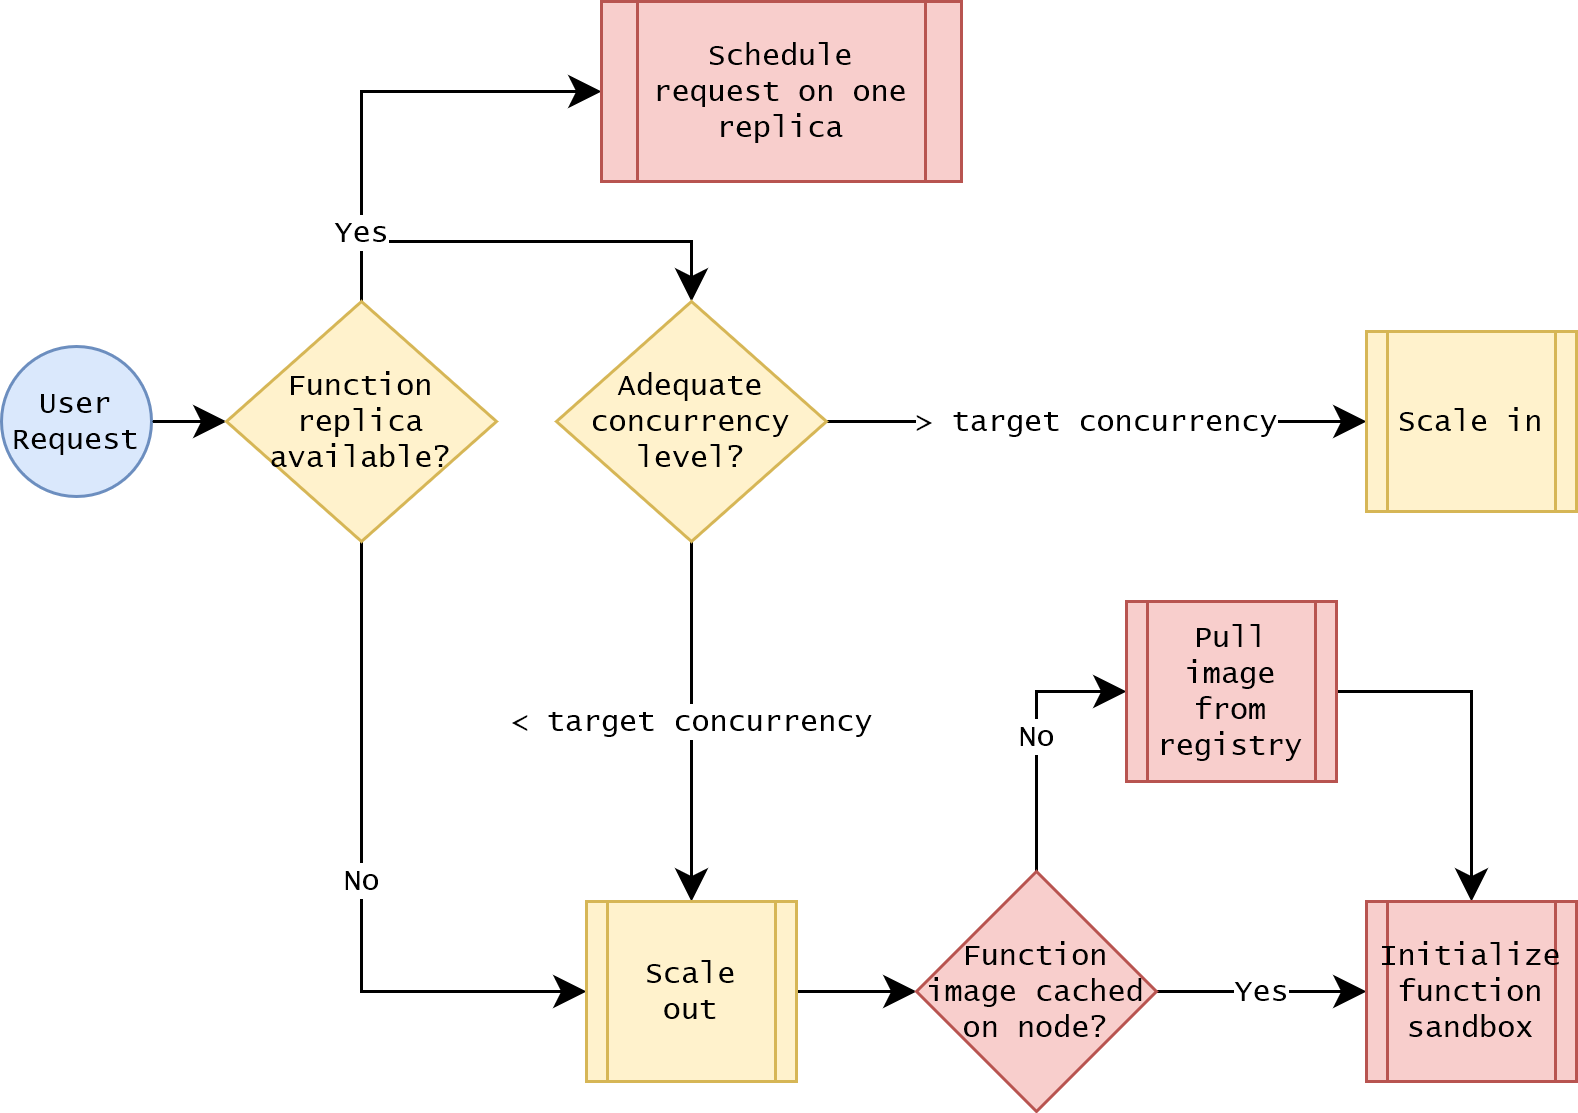
\includegraphics[width=0.8\columnwidth]{6_Chapitre4/figures/function-cache.png}
\caption{Lifecycle of a user request in a serverless platform.}
\label{figure:herocache-function-cache}
\end{figure}

\begin{figure}[t]
\centering
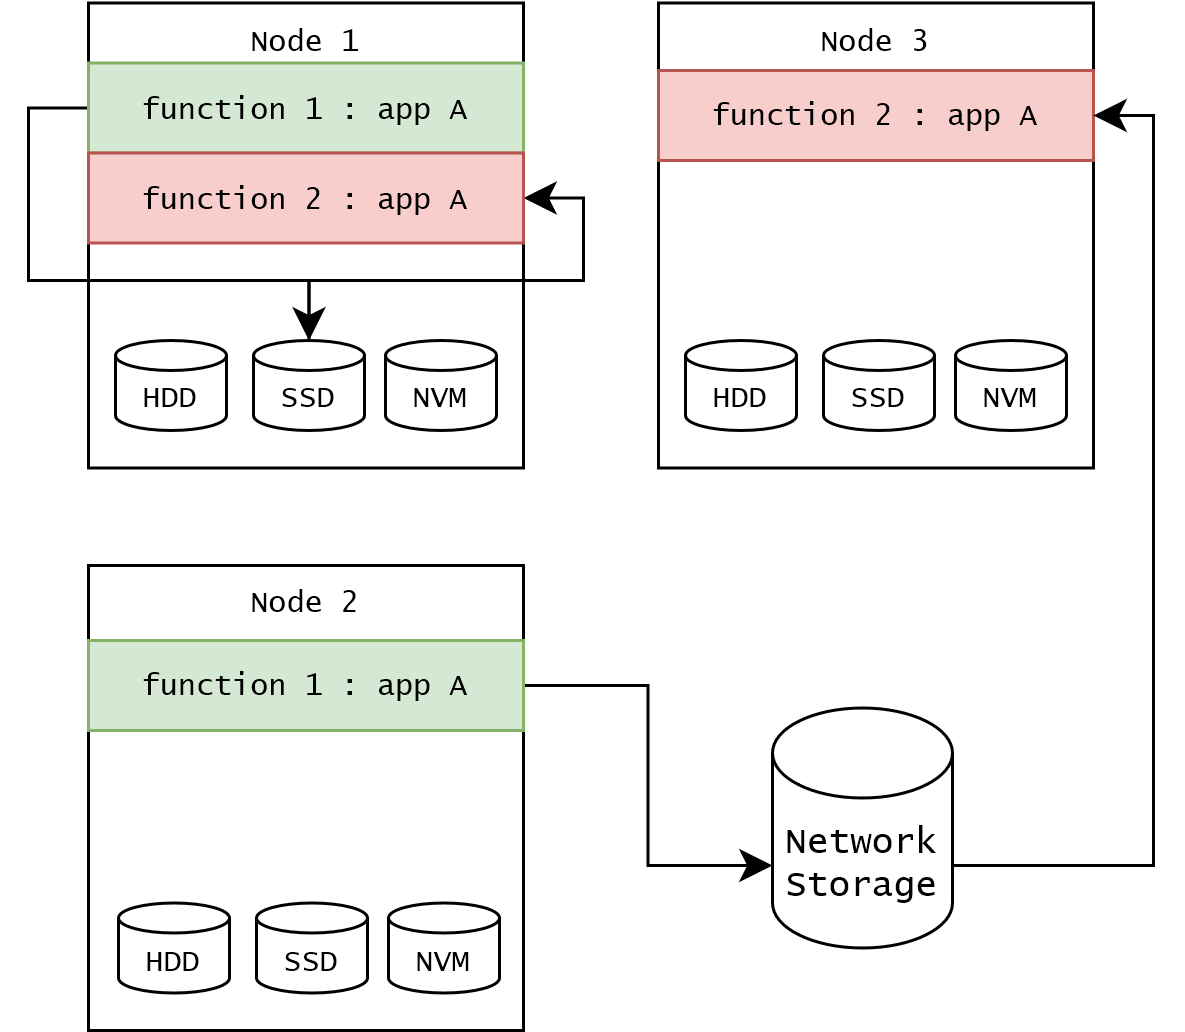
\includegraphics[width=0.8\columnwidth]{6_Chapitre4/figures/function-communications.png}
\caption{Serverless functions communicate intermediate results through persistent storage that can be local to edge nodes or remotely accessible.}
\label{figure:herocache-function-communications}
\end{figure}

\begin{figure*}[t]
\centering
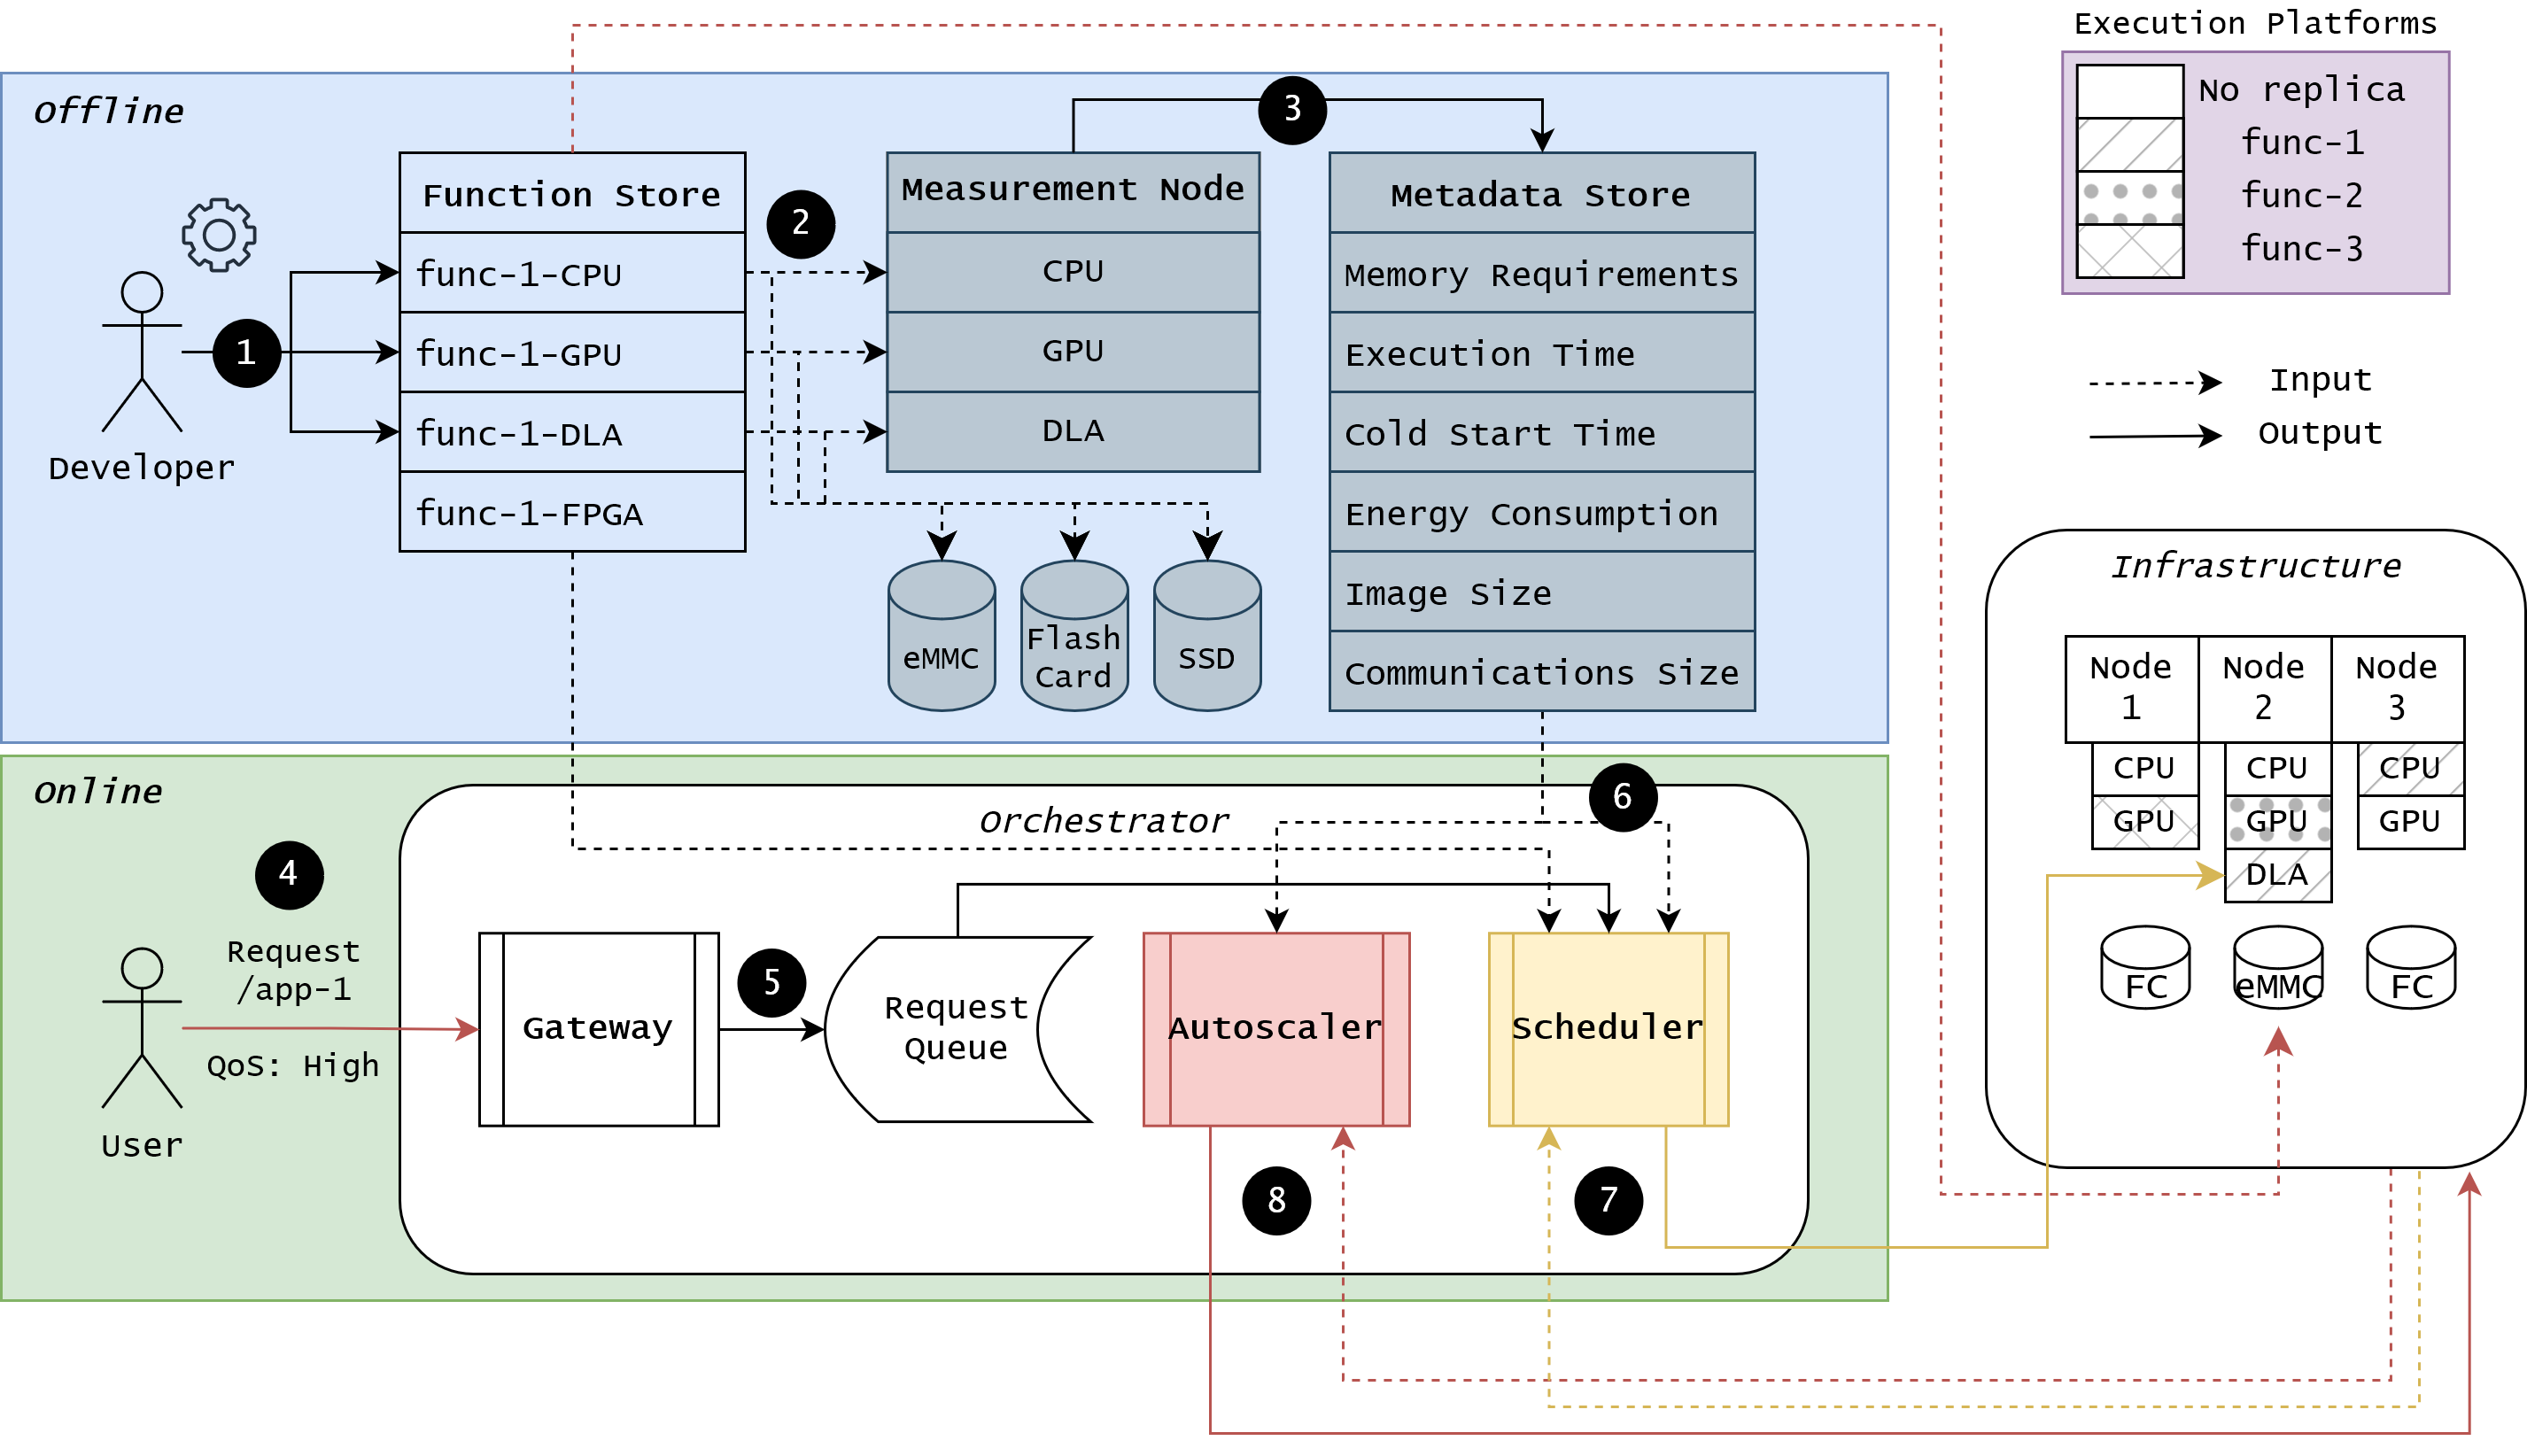
\includegraphics[width=0.65\textwidth]{6_Chapitre4/figures/serverless-platform-storage.png}
\caption{Serverless IDS platform, system overview}
\label{figure:herocache-serverless-platform}
\end{figure*}

\subsection{Défis de l'orchestration dynamique}

Le serverless est un modèle de service tendance pour le cloud~\cite{Lannurien2023} : en transférant la responsabilité de l'allocation des ressources des clients aux fournisseurs de services, il allège une partie importante de la complexité des développeurs d'applications et ouvre de nouvelles possibilités d'optimisation et de contrôle des coûts pour le gestionnaire d'infrastructure.
Dans une architecture serverless, les développeurs conçoivent leurs applications comme une composition de fonctions sans état. Sans état (ou "pur", sans effet secondaire) signifie que le résultat du calcul dépend exclusivement des entrées \cite{burckhardtNetheriteEfficientExecution}. Ces fonctions prennent en entrée une charge utile et un contexte d'invocation, et produisent un résultat qui est stocké dans un niveau de stockage persistant accessible par le réseau. Cela signifie que les dépendances de données entre les fonctions d'une chaîne doivent être gérées par la plateforme.

Lorsqu'un événement déclenche leur exécution, les fonctions sont déployées sur des nœuds de l'infrastructure, dans des environnements d'exécution appelés \textbf{répliques}. Comme les fonctions sont sans état, les demandes peuvent être attribuées à n'importe quelle réplique disponible. La mise à l'échelle d'une application serverless, \textit{i.e.} pour maintenir un niveau de performance constant, consiste à faire croître ou décroître le pool de répliques des fonctions en suivant les pics de charge. Les plateformes serverless basées sur Kubernetes, telles que Knative \cite{knative} ou OpenWhisk \cite{openwhisk}, ont proposé un modèle basé sur le seuil pour le rightsizing du pool de réplicas. Pour toute fonction, un \textit{autoscaler} peut déployer plusieurs \textit{répliques} pour absorber la charge. Chaque réplique est allouée à une plateforme d'exécution (\textit{e.} un cœur de CPU, un GPU, etc.) et dispose d'une file d'attente de longueur fixe pour les demandes entrantes. Le nombre de répliques pour une fonction donnée à un moment donné détermine son niveau de concurrence. Un ordonnanceur place les demandes des utilisateurs dans la file d'attente des répliques de la fonction. Lorsqu'une réplique n'a plus de demandes, elle est désattribuée. Lorsqu'une fonction est demandée alors qu'aucune réplique n'existe, elle passe par un \textbf{démarrage à froid} qui entraîne un délai d'initialisation du temps de réponse de la fonction.

Dans le serverless, la fréquence des allocations de ressources augmente considérablement par rapport aux environnements à ressources réservées toujours actives, tels que les offres IaaS. La capacité des plateformes serverless à mettre à l'échelle une fonction jusqu'à zéro réplique afin d'éviter de facturer les clients pour des ressources inactives est une différence essentielle par rapport aux modèles de services cloud traditionnels.

Ce démarrage à froid présente un risque d'augmentation de la latence, car le fournisseur doit allouer des ressources matérielles et instancier l'application avant de répondre à la demande. Plus l'application est complexe, plus le risque de retards importants est élevé~\cite{mohanAgileColdStartsa}. Les fournisseurs pré-affectent généralement certaines ressources pour éviter les démarrages à froid, ce qui a un coût en termes de provisionnement des ressources. Les acteurs commerciaux tels qu'AWS, Google et Microsoft réutilisent tous, dans une certaine mesure, des instances de fonction, en les laissant fonctionner pendant une période de temporisation afin de contourner les coûts de latence induits par les démarrages à froid~\cite{vahidiniaColdStartServerless2020}.

Une étude récente a montré que 50\% des applications serverless déployées sur Microsoft Azure Durable Functions \footnote{\href{https://learn.microsoft.com/en-US/azure/azure-functions/durable/durable-functions-overview}{https://learn.microsoft.com/en-US/azure/azure-functions/durable/durable-functions-overview}} sont constituées de 3 fonctions ou moins, 65\% des applications présentant un simple DAG de fonctions agencées sous forme de chaînes linéaires \cite{mahgoubORIONThreeRights}. Notre application IDS se compose de différentes chaînes de deux fonctions, comme décrit dans la section~\ref{section:herocache-characterization-workloads}. Les travaux de caractérisation des charges de travail ont montré que 25\% des fonctions déployées sur Microsoft Azure Functions \footnote{\href{https://azure.microsoft.com/en-us/products/functions/}{https://azure.microsoft.com/en-us/products/functions/}} s'exécutent en 100 ms ou moins \cite{shahradServerlessWildCharacterizing}. Les fonctions qui composent notre application IDS s'exécutent pendant des centièmes ou des dixièmes de seconde, ce qui les rend particulièrement sujettes à des ralentissements critiques dans le contexte de ressources allouées de manière dynamique.

\subsection{Mise en cache des images de fonctions}
\label{section:herocache-background-cache}

En ligne, l'allocation dynamique des ressources et les politiques de placement des tâches peuvent aider à répondre aux exigences de qualité de service (QoS) par demande en attribuant les requêtes aux répliques appropriées dans l'infrastructure. Cependant, la plupart des articles sur l'orchestration des ressources et le placement des tâches dans le serverless ne considèrent que les meilleurs scénarios, dans lesquels les images de fonctions sont déjà disponibles sur les nœuds edge. Cela ne reflète pas la réalité, où les images de fonctions sont stockées dans des registres sur des nœuds dédiés et téléchargées sur les nœuds de calcul lors du déploiement des fonctions. En fonction de la taille de l'image, cela peut avoir des conséquences néfastes sur la latence des requêtes avec des déploiements où les démarrages à froid dominent le temps de réponse total d'une fonction \cite{yanHermesEfficientCache2020}.

Afin de répondre aux demandes des utilisateurs sans dégrader les performances, l'autoscaler ajuste périodiquement le nombre de répliques pour chaque fonction déployée : le pool de répliques croît et décroît en fonction des variations de la charge de l'application. Lorsque la charge d'une fonction augmente au-delà du seuil de concurrence de la plateforme, l'autoscaler crée une nouvelle réplique qui traitera les demandes supplémentaires des utilisateurs. Lorsque la charge diminue, les répliques inactives sont supprimées. S'il n'y a plus de demandes pour une fonction donnée, celle-ci peut être \textit{scaled to zero}, ce qui permet d'éviter le gaspillage des ressources.

Les répliques de fonctions sont initialisées à partir d'\textbf{images de fonctions} (\textit{e.g.} une image Docker). Celles-ci sont stockées dans un registre d'images. Ces registres peuvent être accessibles à distance via l'internet et sont généralement déployés dans l'infrastructure du fournisseur dans le contexte d'un nuage privé. Toutefois, de nombreuses études antérieures \cite{bhasiCypressInputSizesensitive2022, zijunFassflowEfficient2022, smithFaDOFaaSFunctions2022, zhangFIRSTExploitingMultiDimensional2023} n'envisagent que des scénarios optimaux dans lesquels les images de fonctions sont déjà disponibles sur les nœuds edge. Cela ne reflète pas la réalité où les images de fonctions sont stockées dans des registres sur des nœuds dédiés et tirées par les nœuds de bordure où et quand les fonctions sont déployées. En fonction de la taille de l'image, cela peut avoir des conséquences néfastes sur la latence des requêtes, en particulier dans les cas où les démarrages à froid dominent le temps de réponse total d'une fonction.

En fait, l'extraction d'images sur les nœuds edge peut représenter plus de 80\% du temps de réponse d'une fonction \cite{yanHermesEfficientCache2020} puisque la latence du démarrage à froid domine le temps de réponse total de la fonction. Cette situation n'est pas acceptable lorsque la plateforme doit répondre à des exigences strictes en matière de qualité de service, comme c'est le cas pour les tâches critiques telles que l'IDS.

\subsection{Communications entre les fonctions}
\label{section:herocache-background-communications}

En outre, comme ces fonctions sont parfois mises à l'échelle à partir de zéro, elles ne sont pas adressables par le réseau : les communications entre les fonctions sont réalisées par l'utilisation d'un stockage lent et accessible par le réseau (\textit{e.g.} Amazon S3). Cela induit des retards qui peuvent faire boule de neige tout au long de l'exécution de l'application et provoquer des violations de l'objectif de niveau de service (SLO) en augmentant les latences de queue de requête \cite{wawrzoniakBoxerDataAnalytics2021a}. Les offres FaaS sont un exemple typique d'architecture d'expédition de données : des gigaoctets de données sont déplacés vers des mégaoctets de code, ce qui entraîne des inefficacités qui augmentent la consommation d'énergie et la sous-utilisation des ressources.

Comme il est nécessaire de prendre en charge la mise à l'échelle dynamique des fonctions, chaque invocation d'une fonction serverless est autonome et ne porte pas les informations ou le contexte des invocations précédentes. Cela permet aux répliques de mettre en file d'attente les demandes des utilisateurs et de les traiter de manière séquentielle sans avoir besoin de procéder à un démarrage à froid entre les demandes. Cela introduit une contrainte sur la plateforme serverless : si une application est composée de plusieurs fonctions qui forment un pipeline de traitement, la sortie de chaque fonction doit être stockée dans un stockage persistant pour être alimentée en entrée de la fonction suivante dans la chaîne~\cite{mullerLambadaInteractiveData2020}.

Les travaux de l'état de l'art ont montré que les fonctions serverless qui communiquent par le biais d'un stockage distant peuvent subir un ralentissement jusqu'à 11x par rapport aux fonctions utilisant des communications directes \cite{wawrzoniakBoxerDataAnalytics2021a}. Les fonctions de notre application IDS doivent communiquer des résultats intermédiaires à chaque étape du DAG de l'application. Lorsque les fonctions sont déployées sur différents nœuds edge, les communications inter-fonctions devront être réalisées par l'utilisation d'un stockage à distance. Cela introduit des ralentissements qui peuvent faire boule de neige tout au long de l'exécution des fonctions et détériorer la qualité de service de l'ensemble de l'application.

\section{Détection d'intrusion à l'edge dans le modèle serverless}
\label{section:herocache-before-contrib}

Orchestrer des applications serverless tout en atteignant le SLA nécessite de modéliser soigneusement les caractéristiques de l'application et d'en tenir compte lors de l'allocation des ressources et de l'ordonnancement des demandes des utilisateurs sur la plateforme serverless. La figure~\ref{figure:herocache-serverless-platform} donne un aperçu du cycle de vie global d'une requête sur notre plateforme serverless. Il est divisé en deux phases ; une \textbf{phase hors-ligne} qui consiste à caractériser les applications déployées par les utilisateurs sur les plateformes edge, et une \textbf{phase en ligne} où les requêtes vers ces applications sont ordonnancées sur la plateforme.

\textbf{phase hors-ligne}. Dans notre plateforme, le cycle de vie de l'application commence par une phase hors-ligne, au cours de laquelle le développeur fournit le code de ses fonctions pour différentes architectures matérielles (GPU, CPU, DLA, etc.)~\Circled{1}. Ce code est stocké par le fournisseur de services dans un registre de fonctions. Les fonctions sont ensuite déployées sur un nœud de mesure~\Circled{2} où elles sont exécutées pour générer des métadonnées relatives à l'exécution des fonctions sur des nœuds hétérogènes. Les besoins en mémoire, le temps d'exécution, le temps de démarrage à froid, la consommation d'énergie, la taille de la fonction et la taille de la communication pour chaque fonction sont enregistrés dans un magasin de métadonnées~\Circled{3}. L'exécution de la phase hors-ligne est nécessaire une fois pour une fonction donnée sur une plateforme donnée, comme décrit dans la section~\ref{section:herocache-workload}.

\textbf{Phase en ligne}. Les demandes sont envoyées aux applications IDS avec une charge utile de trafic TCP (paquets sérialisés) à analyser~\Circled{4}, et un niveau de qualité de service souhaité associé pour le temps de réponse de la demande. La demande est ajoutée à une file d'attente~\Circled{5} au niveau de l'orchestrateur. Lorsque l'ordonnanceur extrait la demande de la file d'attente, le magasin de métadonnées est interrogé pour récupérer les métadonnées de fonction appropriées~\Circled{6}.

L'ordonnanceur tente alors de trouver une réplique disponible de la première fonction de l'application pour traiter la demande~\Circled{7}. Si une telle réplique n'existe pas encore, il sera demandé à l'autoscaler d'initialiser une nouvelle instance de la fonction~\Circled{8}. Au cours du cycle de vie de l'application, l'autoscaler vérifie périodiquement la charge moyenne de chaque fonction pour ajuster le nombre de répliques déployées sur la plateforme, en fonction du seuil de concurrence fixé par le fournisseur de services.

Lorsque l'application est terminée, elle renvoie à l'utilisateur un vecteur de classification qui indique les probabilités que le trafic soit malveillant, c'est-à-dire qu'il présente les caractéristiques d'une attaque potentielle.

\section{Phase hors-ligne : caractérisation} 
\label{section:herocache-workload}

\begin{figure}[t]
\centering
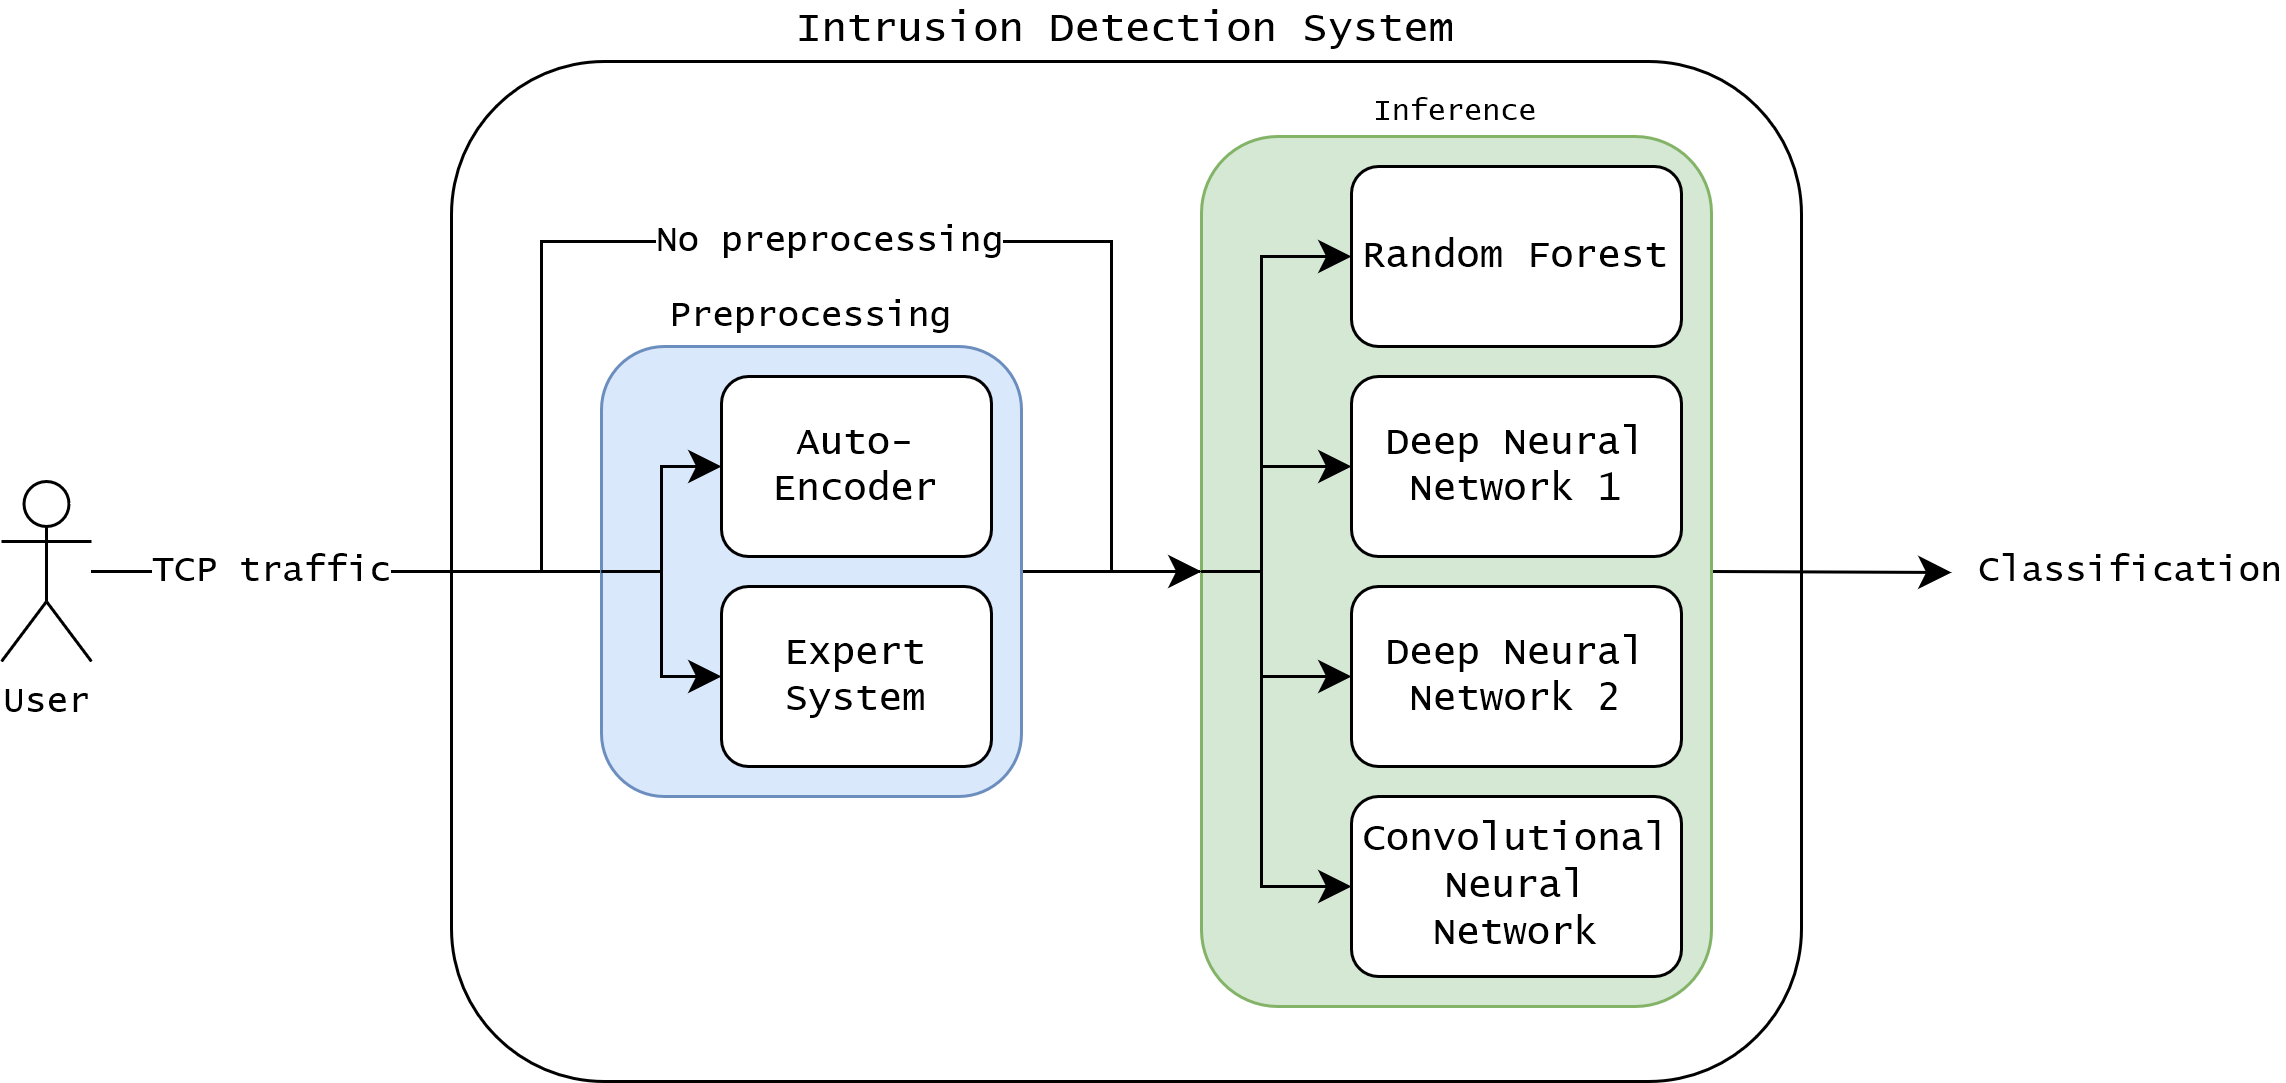
\includegraphics[width=0.8\columnwidth]{6_Chapitre4/figures/ids-application.png}
\caption{Architecture of an IDS application that can make use of different preprocessing functions, and different inference functions to provide the user with a classification of TCP traffic.}
\label{figure:herocache-ids-application}
\end{figure}

Une étape préliminaire de caractérisation de la plateforme et de la charge de travail est nécessaire pour parvenir à une allocation des ressources et à un placement des tâches adéquats pour l'exécution des modèles IDS. À cette fin, nous avons évalué plusieurs modèles IDS en termes de performance et d'énergie sur des plates-formes hétérogènes représentatives des dispositifs edge~\cite{kljucaric2020}. Ces mesures sont cruciales pour une orchestration efficace sur des plates-formes hétérogènes à l'edge. Cette section décrit notre méthodologie et nos résultats.

\subsection{Caractérisation des plateformes d'exécution} \label{section:herocache-characterization-platforms}

Nous avons utilisé des plateformes représentatives de ce que l'on peut trouver en bordure~\cite{slimani:hal-04159551,kljucaric2020} : 
 Il fonctionne sous Linux Raspbian 5.4.
\textbf{(2) Nvidia Jetson Xavier AGX} composé de trois éléments de traitement : un CPU NVIDIA ARM Carmel à 8 cœurs, un GPU NVIDIA Volta avec 512 cœurs CUDA et un accélérateur d'apprentissage profond (DLA), qui est un accélérateur matériel à fonction fixe conçu pour les réseaux neuronaux convolutifs (CNN). Il est supposé être plus économe en énergie que le GPU. Le NVIDIA Xavier AGX est équipé de 16 Go de mémoire LPDDR4 et de 32 Go de mémoire flash eMMC 5.1. Il fonctionne sous Linux Tegra 4.9.10. Le mode d'alimentation 15 Watts Desktop a été utilisé. 
\textbf{(3) PYNQ-Z2 Development Board}, une carte basée sur le système sur puce Xilinx Zynq XC7Z020. Elle est équipée d'un FPGA Artix-7, d'une mémoire DDR3 de 512 Mo et d'une carte SD de 16 Go.

\subsection{Caractérisation des applications}
\label{section:herocache-characterization-workloads}

Notre application se compose de différents préprocesseurs et classificateurs. Le préprocesseur sélectionne un sous-ensemble de caractéristiques pertinentes des paquets TCP. 3 approches de prétraitement différentes ont été utilisées : (1) utilisation de toutes les caractéristiques des paquets sans aucune sélection (NoFS : No Feature Selection) ; (2) utilisation d'un auto-encodeur DNN pour projeter les caractéristiques dans un espace latent plus petit (AE : Auto-Encoder) ; et (3) sélection experte d'un sous-ensemble de caractéristiques (ES : Expert Selection). Pour la partie classification, nous avons utilisé Random Forest (RF), deux architectures différentes de réseaux neuronaux denses (DNN) et un CNN.

\begin{table}[t]
\caption{IDS models architectures and sizes}
\resizebox{\textwidth}{!}{
\begin{tabular}{|c|c|cc|}
\hline
Model     & Architecture                                                                                                                                         & \multicolumn{1}{c|}{Model Size on CPUs (MB)} & Model Size on GPU (MB) \\ \hline
NoFS-RF   & \begin{tabular}[c]{@{}c@{}}5 trees of 100\\ maximum depth\end{tabular}                                                                               & \multicolumn{1}{c|}{28}                      & 15.4                   \\ \hline
AE-RF     & \begin{tabular}[c]{@{}c@{}}5 trees of 50 \\ maximum depth\end{tabular}                                                                               & \multicolumn{1}{c|}{-}                       & 32.9                   \\ \hline
ES-RF     & \begin{tabular}[c]{@{}c@{}}10 trees of 10 \\ maximum depth\end{tabular}                                                                              & \multicolumn{1}{c|}{9.1}                     & 5.5                    \\ \hline
NoFS-DNN1 & \multirow{3}{*}{\begin{tabular}[c]{@{}c@{}}4 Dense Layers \\ (128x64x32x10)\end{tabular}}                                                            & \multicolumn{2}{c|}{0.144}                                            \\ \cline{1-1} \cline{3-4} 
AE-DNN1   &                                                                                                                                                      & \multicolumn{2}{c|}{0.321}                                            \\ \cline{1-1} \cline{3-4} 
ES-DNN1   &                                                                                                                                                      & \multicolumn{2}{c|}{0.053}                                            \\ \hline
NoFS-DNN2 & \multirow{3}{*}{\begin{tabular}[c]{@{}c@{}}5 Dense Layers \\ (7024x704x288x64x10)\end{tabular}}                                                      & \multicolumn{2}{c|}{3.33}                                             \\ \cline{1-1} \cline{3-4} 
AE-DNN2   &                                                                                                                                                      & \multicolumn{2}{c|}{2.96}                                             \\ \cline{1-1} \cline{3-4} 
ES-DNN2   &                                                                                                                                                      & \multicolumn{2}{c|}{2.61}                                             \\ \hline
NoFS-CNN  & \multirow{3}{*}{\begin{tabular}[c]{@{}c@{}}2 Conv1D (x64) - MaxPool \\ 3 Conv1D (x256) - MaxPool\\ 3 Dense Layers (100x20x10)\end{tabular}} & \multicolumn{2}{c|}{4.77}                                             \\ \cline{1-1} \cline{3-4} 
AE-CNN    &                                                                                                                                                      & \multicolumn{2}{c|}{2.9}                                              \\ \cline{1-1} \cline{3-4} 
ES-CNN    &                                                                                                                                                      & \multicolumn{2}{c|}{2.6}                                              \\ \hline
\end{tabular}
}
\label{table:herocache-workload}
\end{table}

Le tableau~\ref{table:herocache-workload} présente les modèles IDS pris en compte dans cette étude et certaines de leurs caractéristiques. Ces modèles ont été formés et caractérisés sur l'ensemble de données de référence sur les intrusions dans le réseau UNSW-NB15\footnote{\href{https://research.unsw.edu.au/projects/unsw-nb15-dataset}{https://research.unsw.edu.au/projects/unsw-nb15-dataset}}
où chaque observation représente des caractéristiques statistiques, de contenu et de temps sur le trafic de données au cours d'une fenêtre temporelle, et est étiquetée comme "normale" ou "attaque". L'ensemble de données comprend 9 catégories d'attaques. Les modèles de réseaux neuronaux ont été exportés et optimisés à l'aide de TensorFlow Lite et TensorRT lorsqu'ils étaient destinés à des plateformes CPU et GPU/DLA, respectivement. En ce qui concerne Random Forest, les modèles ont été exportés en utilisant les frameworks Emlearn et HummingBird.ml lorsqu'ils étaient destinés aux plateformes CPU et GPU, respectivement. hls4ml a été utilisé pour exporter les modèles de réseaux neuronaux pour la cible FPGA.

\subsection{Mesures de performances}

Chacun des modèles IDS a été déployé sur les plateformes cibles et les inférences ont été exécutées avec un ensemble de 80 000 paquets provenant de l'ensemble de données UNSW-NB15 afin de caractériser la latence d'inférence. Les résultats sont présentés dans la figure~\ref{figure:herocache-performance}. Seul un modèle (ES-DNN1) a été caractérisé sur la plateforme FPGA car les autres modèles HLS n'ont pas pu être pris en compte sur la cible. La conclusion qui a été tirée de ces résultats est que pour les réseaux neuronaux, le CPU Xavier atteint la meilleure performance dans la majorité des cas, à l'exception de NoFS-CNN qui profite des capacités du GPU en raison de son nombre élevé de paramètres et de l'efficacité du GPU pour les opérations de convolution. Pour les modèles Random Forest, l'élément de traitement le plus rapide est le GPU. En termes de coût et de disponibilité, la Xavier AGX est respectivement environ 20x et 10x plus chère que les plateformes RBPI4 et Pynq-Z2. Nous dimensionnons notre infrastructure en conséquence en fournissant plus de plateformes RBPI4 que de Xavier AGX pour être représentatifs des déploiements réels.

\begin{figure}
    \centering
    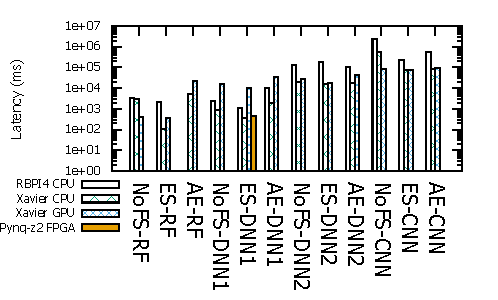
\includegraphics[width=0.9\columnwidth]{6_Chapitre4/figures/latency_bar.pdf}
    \caption{Latency characterization of IDS models.}
    \label{figure:herocache-performance}
\end{figure}

\subsection{Mesures de consommation d'énergie}

Nous avons exécuté des inférences sur les modèles IDS sur chaque élément de traitement et mesuré la consommation d'énergie de la plateforme à l'aide de l'analyseur de puissance N6705A DC. Les résultats sont présentés dans la figure~\ref{figure:herocache-energy}. Pour les mêmes raisons que celles mentionnées ci-dessus, seul ES-DNN1 a été caractérisé sur FPGA. Nous observons que les éléments de traitement du CPU affichent une consommation d'énergie inférieure à celle du GPU dans la majorité des cas. Le seul cas où le GPU obtient de meilleurs résultats est lorsque la vitesse qu'il atteint par rapport aux CPU est élevée. C'est par exemple le cas pour NoFS-CNN, où le CPU RBPI4 est plus de 30 fois plus lent que le GPU. Même si Pynq-Z2 présente la meilleure efficacité énergétique avec le modèle ES-DNN1, étant donné qu'il est plus cher et présente une générosité de conception limitée, nous supposons qu'il est moins disponible que le RBPI4.

\begin{figure}
    \centering
    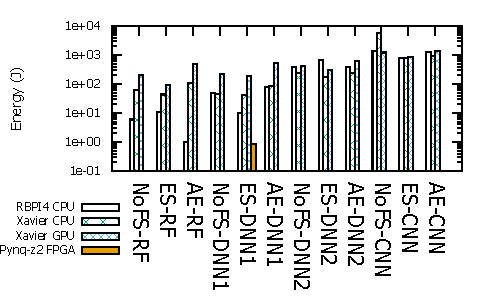
\includegraphics[width=0.9\columnwidth]{6_Chapitre4/figures/energy_bar.pdf}
    \caption{Energy characterization of IDS models.}
    \label{figure:herocache-energy}
\end{figure}

\section{Phase en ligne : orchestration avec HeROcache} \label{section:herocache-contribution}

\subsection{Présentation générale}

L'orchestrateur HeROcache est principalement composé de deux modules, le \textbf{autoscaler} et le \textbf{scheduler} (voir figure~\ref{figure:herocache-serverless-platform}). L'autoscaler est chargé de l'allocation dynamique des ressources : il affecte les plateformes d'exécution aux répliques de fonctions. L'ordonnanceur s'occupe du placement des demandes des utilisateurs sur les répliques.

HeROcache relève les trois défis susmentionnés en concevant des stratégies complémentaires de minimisation des coûts au niveau de l'autoscaler et de l'ordonnanceur. HeROcache minimise \textbf{les délais d'initialisation} en tenant compte des temps de latence de l'extraction d'images au niveau de l'autoscaler. Des stratégies d'extraction préalable sont également mises en œuvre pour la mise en cache des images de fonctions. Les coûts de \textbf{communication interfonction} sont pris en compte principalement dans la partie de l'ordonnanceur, qui tend naturellement à consolider les fonctions d'une même application. L'autoscaler participe indirectement à cette consolidation en préemptant les fonctions suivantes du DAG de l'application sur le même nœud de bordure. Enfin, \textbf{plateformes hétérogènes} sont prises en compte car les différents coûts d'exécution extraits pendant la phase hors-ligne (voir Section~\ref{section:herocache-workload}) sont pris en compte tout au long du processus d'autoscaling et d'ordonnanceur. Les sections suivantes décrivent les stratégies de mise à l'échelle automatique et d'ordonnanceur.

\begin{table}[t]
    \caption{Notation dictionary}
    \begin{center}
    \scalebox{0.85}{\begin{tabularx}{\linewidth}{|c|Y|}
    \hline
    \textbf{Notation} & \textbf{Description} \\ \hline
    $x_a$ & Allocation of resource for application $a$ \\ \hline
    $y_a$ & Invocation of application $a$ \\ \hline
    $z_i$ & Placement of task for function $i$ \\ \hline
    $f_{N, P}$ & A function $f$ scheduled to run on a platform $P$ available on node $N$ \\ \hline
    $f_{a}$ & A function $f$ that belongs to application $a$ \\ \hline
    $A$ & Total number of applications to be scheduled on the platform \\ \hline
    $F_{a}$ & Total number of functions that belong to an application $a$ \\ \hline
    $RT_{{f}_{N, P}}$ & Time to retrieve function image for $f$ to run on a platform $P$ available on node $N$ \\ \hline
    $NB_{N}$ & Network bandwidth between node $N$ and the infrastructure \\ \hline
    $SMT_{N}$ & Storage medium throughput on node $N$ \\ \hline
    $SML_{N}$ & Storage medium latency on node $N$ \\ \hline
    $QP$ & QoS penalty \\ \hline
    $QD$ & QoS deviation \\ \hline
    $WET$ & Worst execution time \\ \hline
    $TT$ & Task total time \\ \hline
    $CST$ & Cold start time \\ \hline
    $ST$ & Storage time \\ \hline
    $ET$ & Execution time \\ \hline
    $EC$ & Energy consumption \\ \hline
    $IS$ & Image size \\ \hline
    $HP$ & Hardware price \\ \hline
    $TC$ & Task consolidation \\ \hline
    $Q$ & Task queue on a replica \\ \hline
    $CP$ & Cache proportion \\ \hline
    $SIS^{f}_{a}$, $SOS^{f}_{a}$ & Size of resp. input, output state of function $f$ that belongs to application $a$ \\ \hline
    $threshold_{f, h}$ & Concurrency threshold for a function $f$ on a replica of hardware type $h$ \\ \hline
    $scaleCost^{{f}_{{i}_{N, P}}}_a$ & Cost of creating a new replica for function $f_i$ from application $a$ on a platform $P$ available on node $N$ \\ \hline
    $schedCost^{{f}_{{i}_{N, P}}}_a$ & Cost of scheduling an execution of function $f$ from application $a$ on a platform $P$ available on node $N$ \\ \hline
    \end{tabularx}}
    \label{table:herocache-notation}
    \end{center}
\end{table}

\subsection{Stratégie de minimisation des coûts d'allocation des ressources}

Nous formulons l'allocation des ressources comme un problème d'optimisation et nous le résolvons à l'aide d'un algorithme gourmand simple. L'objectif de l'autoscaler est de minimiser le coût de la somme des allocations $scaleCost_{a}$ pour $y_a$ invocations de l'application $a$ (équation~\ref{eq:herocache-objective-allocation}) pour toutes les applications dans $A$, sous la contrainte d'une infrastructure finie avec $x_a$ étant l'allocation de ressources pour l'application $a$ (équation~\ref{eq:herocache-constraint-allocation}). 

\begin{equation}
    \forall A, \, \min \sum_{a = 0}^{A} y_a \cdot scaleCost_{a}
\label{eq:herocache-objective-allocation}
\end{equation}

\begin{equation}
    \text{s. t.} \, \sum_{a = 0}^{A} x_a \leq Total Resources
\label{eq:herocache-constraint-allocation}
\end{equation}

Le coût de l'allocation des ressources pour une application $a$ est la somme des coûts d'allocation de ses fonctions (équation~\ref{eq:herocache-scale-cost-app}). Une réplique est allouée à une plateforme d'exécution.

\begin{equation}
    scaleCost_{a} = \, \sum_{i = 0}^{F_{a}} scaleCost^{{f}_{{i}_{N, P}}}_a
\label{eq:herocache-scale-cost-app}
\end{equation}

Chaque réplique de fonction a un coût d'allocation associé, car l'allocation dynamique des ressources matérielles introduit un temps de latence lors du traitement des demandes des utilisateurs. 

Nous avons conçu un modèle de coût (équation~\ref{eq:herocache-scale-cost-function}) pour l'allocation des ressources nécessaires au déploiement d'une fonction d'une application donnée. Il est composé de quatre éléments, dont nous devons minimiser la somme :

\begin{itemize}
    \item La \textit{proportion de cache} $CP$ traduit la dispersion des fonctions sur les différents nœuds de bordure. Plus le score est élevé, plus les fonctions sont dispersées sur les nœuds. La minimisation de ce terme permet de consolider les fonctions ;
    \item Le \textit{temps total} $TT$ représente le temps d'exécution total de la fonction. Il tient compte de la qualité de service de l'application, de l'hétérogénéité de la plateforme et du coût de déploiement (si l'image est mise en cache ou distante). Plus ce coût est élevé, plus la qualité de service est faible ;
    \item La \textit{consommation d'énergie} $EC$ traduit la consommation d'énergie du déploiement de la fonction. Plus $EC$ est élevé, plus le coût est important ;
    \item Le \textit{prix du matériel} $HP$ décrit le coût total de possession (TCO) supporté par les fournisseurs de services en fonction du temps d'exécution. Il traduit le coût de déploiement sur une plateforme matérielle donnée. Plus $HP$ est élevé, plus le coût de la solution est important.
\end{itemize}

L'objectif global du modèle de coût est de déployer une fonction au coût le plus bas possible, c'est-à-dire une consolidation accrue, une réduction du makespan, une réduction de la consommation d'énergie et une réduction du coût de possession. Nous détaillerons chaque partie de l'équation~\ref{eq:herocache-scale-cost-function} dans les paragraphes suivants. Chaque composante de l'équation est pondérée pour permettre un réglage souple ; les valeurs que nous avons choisies pour le déploiement de l'application IDS sont spécifiées dans la partie consacrée à l'évaluation (Section~\ref{section:herocache-evaluation}).

\begin{equation}
\begin{split}
 \forall N, \forall P \in N, scaleCost^{{f}_{{i}_{N, P}}}_{a} = \,   &k_{CP} \cdot {CP}_{{a}_{N}}    \\
    + &k_{TT} \cdot {TT}_{{f}_{N, P}} \\
    + &k_{EC} \cdot {EC}_{{f}_{N, P}} \\
    + &k_{HP} \cdot {HP}_{{f}_{N, P}}
\end{split}
\label{eq:herocache-scale-cost-function}
\end{equation}

\textbf{Proportion de cache}. Comme nous l'avons vu précédemment, l'application de la consolidation des tâches (exécution d'une fonction) entre les applications devrait permettre de minimiser la communication et les retards dans les chaînes de fonctions. HeROcache favorise le déploiement de répliques d'une fonction sur des nœuds où d'autres fonctions appartenant à la même application sont déjà déployées.

Pour ce faire, HeROcache suit $CF_{a}^{{f}_{i_{N, P}}}$ le nombre d'images de fonctions ${f}_{i}$ de l'application $a$ déployée sur le nœud $N$ sur une plateforme d'exécution donnée $P$ (par exemple, GPU) disponible en cache sur le stockage local du nœud. La proportion de fonctions mises en cache est calculée pour chaque application (équation~\ref{eq:herocache-cached-functions}), puis la moyenne est calculée sur toutes les applications s'exécutant sur un nœud donné et inversée pour donner une valeur élevée aux fonctions non consolidées (l'objectif étant de minimiser cette proportion), voir équation~\ref{eq:herocache-cache-proportion-app}.

\begin{equation}
    \forall a \in A, \, \forall f \in a, \, CF_{a}^{{f}_{i_{N, P}}} = \frac{\sum_{i = 0}^{Fa} isCached(f_{i}, N, P)}{F_{a}}
\label{eq:herocache-cached-functions}
\end{equation}

\begin{equation}
    \forall N, \forall P \in N, \, {CP}_{{a}_{N}} = \, \frac{A}{\sum_{i = 0}^{F_{a}} CF_{a}^{{f}_{i_{N, P}}}}
\label{eq:herocache-cache-proportion-app}
\end{equation}

En plus de la minimisation des coûts, afin de réduire les délais de déploiement, l'autoscaler préfigure les images des chaînes de fonctions lors du déploiement d'une nouvelle réplique sur un nœud. Il inspecte les chaînes de fonctions et extrait séquentiellement les images de fonctions manquantes du registre distant vers le stockage local du nœud de manière asynchrone.

\textbf{Temps total}. La deuxième composante du coût de mise à l'échelle est le \textit{temps total}. La minimisation du temps total devrait empêcher les retards d'initialisation de faire boule de neige dans les chaînes de fonctions, évitant ainsi les violations des accords de niveau de service (SLA).

Grâce aux métadonnées collectées sur chaque fonction pendant la phase hors-ligne, l'autoscaler est en mesure de prédire le temps total ${TT}_{{f}_{N, P}}$ de la première requête qui sera ordonnancée sur une nouvelle réplique de fonction (équation~\ref{eq:herocache-total-time-function}).

\begin{equation}
    {TT}_{{f}_{N, P}} = \, {RT}_{{f}_{N, P}} + {WT}_{{f}_{N, P}} + {CST}_{{f}_{N, P}} + {ET}_{{f}_{N, P}}
\label{eq:herocache-total-time-function}
\end{equation}

\begin{itemize}
    \item ${RT}_{{f}_{N, P}}$ est la durée du temps de récupération de l'image de la fonction. Si l'image de la fonction est déjà mise en cache sur le nœud de calcul, cette durée est nulle ; sinon, elle dépend de la taille de l'image $IS$ et est influencée par la largeur de bande de la liaison réseau $NB$, car l'image sera lue à partir d'un registre d'images distant, et par le débit du support de stockage du nœud $SMT$ et la latence $SML$, car l'image sera écrite et stockée localement en vue d'une utilisation ultérieure (équation~\ref{eq:herocache-retrieval-time}) ;

    \begin{equation}
        {RT}_{{f}_{N, P}} = \, \frac{IS_{{f}_{N, P}}}{\min (NB_{N}, SMT_{N})} + SML_{N}
        \label{eq:herocache-retrieval-time}
    \end{equation}

    \item ${WT}_{{f}_{N, P}}$ est le temps que la tâche passera à attendre dans la file d'attente de la plateforme. Au moment de la création de la réplique, ce temps sera égal à zéro car nous ne prévoyons que la latence de la première requête sur la réplique ;
    \item ${CST}_{{f}_{N, P}}$ est le temps de démarrage à froid nécessaire pour initialiser l'instance de la fonction (\textit{i.e.} décompresser l'image, préparer le conteneur, initialiser les bibliothèques, etc. Il est mesuré en fonction des métadonnées extraites ;
    \item ${ET}_{{f}_{N, P}}$ est la durée d'exécution de la fonction, y compris le temps de communication avec ses prédécesseurs et successeurs potentiels dans le DAG. Cette durée tient compte de l'extraction des métadonnées de la plateforme (équation~\ref{eq:herocache-execution-time}).
\end{itemize}

\begin{equation}
    {ET}_{{f}_{N, P}} = \, {CT}_{{f}_{N, P}} + {ST}_{{f}_{N, P}}
\label{eq:herocache-execution-time}
\end{equation}

${CT}_{{f}_{N, P}}$ est le \textit{temps de calcul} de la fonction -- le temps attendu pour que la fonction termine son exécution une fois entièrement initialisée. La valeur dépend des performances et de la disponibilité de la plateforme d'exécution. ${ST}_{{f}_{N, P}}$ est le \textit{temps de stockage} de la fonction -- le temps attendu pour que la fonction récupère ses données d'entrée et stocke ses données de sortie. La valeur dépend des performances de la liaison réseau et des dispositifs de stockage.

Le temps de stockage de la fonction ${ST}_{{f}_{N, P}}$ dépend de la taille de son état, \textit{c.-à-d.} de ses données d'entrée et de sortie. La récupération de l'entrée et le stockage de la sortie de chaque fonction de la chaîne dépendent des performances de la liaison réseau et du débit et de la latence du support de stockage sélectionné, comme le montre l'équation~\ref{eq:herocache-storage-time}.

\begin{equation}
    {ST}_{{f}_{N, P}} = \, \frac{SIS_{a}^{f_{i_{N, P}}} + SOS_{a}^{f_{i_{N, P}}}}{\min (NB_{N}, SMT_{N})} + SML_{N}
\label{eq:herocache-storage-time}
\end{equation}

\textbf{Consommation d'énergie et prix du matériel}. Enfin, la prise en compte de la consommation d'énergie et du prix du matériel devrait permettre de départager les candidats lorsque plusieurs allocations possibles semblent produire le même coût (en fournissant le même niveau de qualité de service).

${EC}_{{f}_{N, P}}$ et ${HP}_{{f}_{N, P}}$ correspondent respectivement (a) à la consommation d'énergie dynamique générée par cette allocation obtenue grâce à la phase de caractérisation hors-ligne de la charge de travail et de la plateforme et (b) au prix de détail suggéré par le fabricant (MSRP) du matériel mobilisé $Hardware Price_{P}$ pour déployer la fonction sur ledit nœud et ladite plateforme au regard du temps d'exécution de la fonction $ET_{{f}_{N, P}}$ (équation~\ref{eq:herocache-hardware-price}).

\begin{equation}
    {HP}_{{f}_{N, P}} = \frac{Hardware Price_{P}}{ET_{{f}_{N, P}}}
\label{eq:herocache-hardware-price}
\end{equation}

\subsection{Stratégie de minimisation des coûts d'ordonnancement et de placement des données}

Comme pour l'autoscaling, nous formulons un problème d'optimisation pour trouver la configuration d'ordonnancement optimale pour chaque demande d'utilisateur (puisque la qualité de service doit être garantie sur la base d'une demande d'utilisateur) et nous le résolvons à l'aide d'un simple algorithme d'avidité. L'objectif de l'ordonnanceur est de minimiser le coût du placement de $z_i$ tâches sur $R_i$ répliques de la fonction $i$ pour $y_a$ invocations de l'application $a$ (équation~\ref{eq:herocache-objective-scheduling}), sous la contrainte d'un ensemble fini de répliques de fonctions $R_{i}$ (équation~\ref{eq:herocache-constraint-scheduling}) précédemment déployées par l'autoscaler. Nous supposons que les applications sont toujours exécutées jusqu'au bout et que les nœuds ne tombent pas en panne ; il n'y a donc pas de coût associé aux migrations de tâches ou aux nouvelles tentatives.

\begin{equation}
    \min \sum_{a = 0}^{A} y_a \cdot schedCost_{a}
\label{eq:herocache-objective-scheduling}
\end{equation}

\begin{equation}
    \text{s. t.} \, \forall a \sum_{i = 0}^{F_a} z_i \leq \sum_{i = 0}^{F_a} R_{i}
\label{eq:herocache-constraint-scheduling}
\end{equation}

Comme la plateforme fonctionne à la granularité des fonctions, le coût d'ordonnancement d'une application $a$ est la somme du coût d'ordonnancement de sa chaîne de fonctions (équation~\ref{eq:herocache-scheduling-cost-app}).

\begin{equation}
    schedCost_{a} = \, \sum_{i = 0}^{A} schedCost^{{{f}_{i}}}_{a}
\label{eq:herocache-scheduling-cost-app}
\end{equation}

Chaque fonction ordonnancée dans la chaîne a un coût associé calculé pour chaque placement possible sur une réplique existante.
Nous avons conçu un modèle de coût (équation~\ref{eq:herocache-scheduling-cost-function}) pour le placement des tâches nécessaires à l'exécution d'une demande d'utilisateur pour une application. 

\begin{equation}
    schedCost_{{f}_{{i}_{N, P}}} = \, k_{QP} \cdot QP_{{f}_{N, P}} + k_{EC} \cdot {EC}_{{f}_{N, P}} + k_{TC} \cdot TC_{{f}_{N, P}}
\label{eq:herocache-scheduling-cost-function}
\end{equation}

Elle est composée de trois éléments, dont nous devons minimiser la somme :

\begin{itemize}
    \item La \textit{pénalité de qualité de service} $QP$ est encourue par le fournisseur de services lorsqu'une demande d'utilisateur n'est pas traitée en temps voulu. Il s'agit d'une valeur booléenne qui détermine si, en raison d'un placement donné, l'application ne respectera pas son échéance ;
    \item La \textit{consommation d'énergie} $EC$ traduit la consommation d'énergie dynamique induite par l'exécution de la fonction. Plus $EC$ est élevée, plus le coût est important ;
    \item La \textit{consolidation des tâches} $TC$ décrit l'utilisation des ressources pour un placement donné. Plus $TC$ est faible, plus la file d'attente de la réplique est proche de son seuil de concurrence, ce qui maximise l'utilisation du matériel.
\end{itemize}

L'objectif global du modèle de coût est de placer les tâches dans les répliques de fonctions au coût le plus bas possible, c'est-à-dire en évitant les pénalités subies par le fournisseur de services en cas de dépassement du délai de l'application fixé par la demande de l'utilisateur, en utilisant les plates-formes d'exécution les moins gourmandes en énergie possible et en appliquant un ratio d'utilisation élevé pour les ressources allouées à chaque fonction. Nous décrivons chaque partie de l'équation~\ref{eq:herocache-scale-cost-function} dans les paragraphes suivants. Chaque composante de l'équation est pondérée pour permettre un réglage flexible ; les valeurs que nous avons choisies pour le déploiement de l'application IDS sont spécifiées dans la partie consacrée à l'évaluation (Section~\ref{section:herocache-evaluation}).

\textbf{Pénalité de qualité de service}. L'ordonnanceur sélectionne les tâches entrantes en fonction de \textbf{l'échéance la plus proche d'abord}, en s'appuyant sur les métadonnées de la fonction pour calculer un temps d'exécution dans le pire des cas noté $WET$ (équation~\ref{eq:herocache-task-wet}). La demande de l'utilisateur est associée à un niveau de qualité de service qui définit un écart de qualité de service variable $QD$ appliqué au temps d'exécution de l'application. Il s'agit du délai d'exécution de la demande.

\begin{equation}
    \forall \, (N, P), \, WET_{f} = \, \max ET_{f_{N, P}}
\label{eq:herocache-task-wet}
\end{equation}

Nous pouvons prédire la pénalité de l'application en additionnant le temps total prévu pour ses tâches et en le comparant à l'échéance de l'application (somme des échéances des fonctions), voir équation~\ref{eq:herocache-scheduling-penalty}. Nous réutilisons l'équation~\ref{eq:herocache-total-time-function} pour calculer le temps total d'exécution d'une fonction ; cependant, ici, $RT$ et $CST$ seront nuls car la réplique a déjà été initialisée par l'autoscaler lors de l'allocation. $WT$ sera égal à la somme des temps d'exécution des tâches de priorité supérieure actuellement en file d'attente sur la réplique.

\begin{equation}
   QP_{a} = \, \sum_{i = 0}^{F_a} TT_{{f}_{{i}_{N, P}}} > \sum_{i = 0}^{F_a} WET_{f_{i}} \cdot QD_{a}
\label{eq:herocache-scheduling-penalty}
\end{equation}

En prenant en compte le temps de stockage dans le coût d'ordonnancement, nous cherchons à inciter l'ordonnanceur à placer les tâches aussi près que possible des données sur lesquelles elles opèrent. Pour éviter de saturer le stockage local des nœuds, la plateforme procède au nettoyage des données intermédiaires dès que l'application a terminé son exécution, \textit{i.e.} lorsque la dernière fonction de la chaîne renvoie sa valeur.

\textbf{Consommation d'énergie}. ${EC}_{{f}_{N, P}}$ correspond à la consommation d'énergie dynamique générée par cette configuration d'ordonnancement. Elle est liée au temps d'exécution de la fonction. Les résultats des mesures hors-ligne sont utilisés pour ce terme.

\textbf{Consolidation des tâches}. Nous voulons que les files d'attente des répliques de fonctions atteignent leur longueur maximale : le pire cas est d'avoir une file d'attente vide, ce qui signifie que des ressources matérielles auraient été allouées pour rien. Nous voulons également empêcher les files d'attente de répliques de croître trop rapidement au-delà de ce seuil, car cela pourrait entraîner des violations de la qualité de service en raison de longs temps d'attente.

Nous commençons par établir le ratio d'\textit{utilisation de la plateforme} $PU$ de chaque réplique pour la fonction que nous essayons d'ordonnancer (équation~\ref{eq:herocache-platform-usage}) : plus la longueur de la file d'attente de la réplique $Q$ est proche du seuil de concurrence ($threshold$ dans l'équation), plus le score est faible. 

\begin{equation}
    PU_{f_{N, P}} = \frac{Q_{N, P}}{threshold_{f, P}}
\label{eq:herocache-platform-usage}
\end{equation}

Ensuite, nous calculons un score de consolidation des tâches $TC$ en appliquant une fonction exponentielle à $PU$ (équation~\ref{eq:herocache-task-consolidation}). Ainsi, $TC$ est le plus faible pour les placements dans les répliques inactives, et ce coût augmente fortement au fur et à mesure que les files d'attente se remplissent, ce qui conduit l'ordonnanceur à donner la priorité aux placements sur les répliques vides et à ne pas tenir compte des répliques où la file d'attente des requêtes est saturée.

\begin{equation}
    TC_{{f}_{N, P}} = \, exp(PU_{f_{N, P}})
\label{eq:herocache-task-consolidation}
\end{equation}

\section{Évaluation}
\label{section:herocache-evaluation}

Cette section présente notre méthodologie d'évaluation et les résultats obtenus dans un scénario de déploiement d'IDS sur des dispositifs edge. L'évaluation se fait en deux phases : nous comparons HeROcache à plusieurs lignes de base, puis nous évaluons l'impact de chacun de ses composants (autoscaler et ordonnanceur) pris séparément.

\begin{figure*}[t]
    \center
    \subfloat[Consolidation\label{figure:herocache-evaluation-full-unused-nodes}]{
        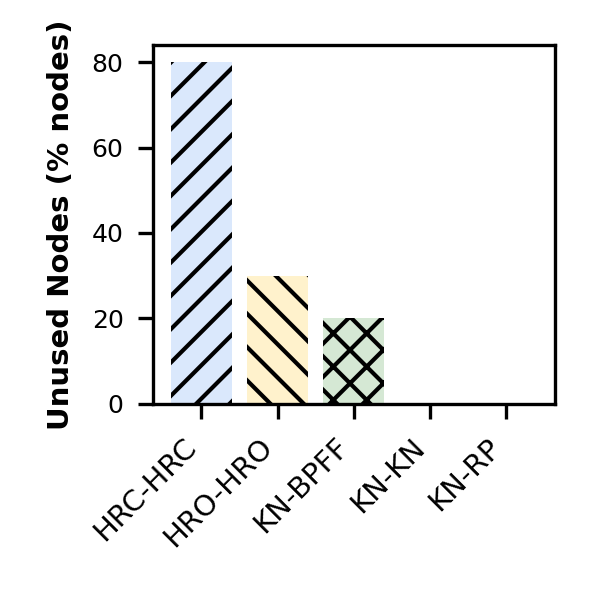
\includegraphics[width=0.155\linewidth]{6_Chapitre4/figures/eval/2-unused-nodes.png}
    }
    \subfloat[QoS\label{figure:herocache-evaluation-full-penalty}]{
        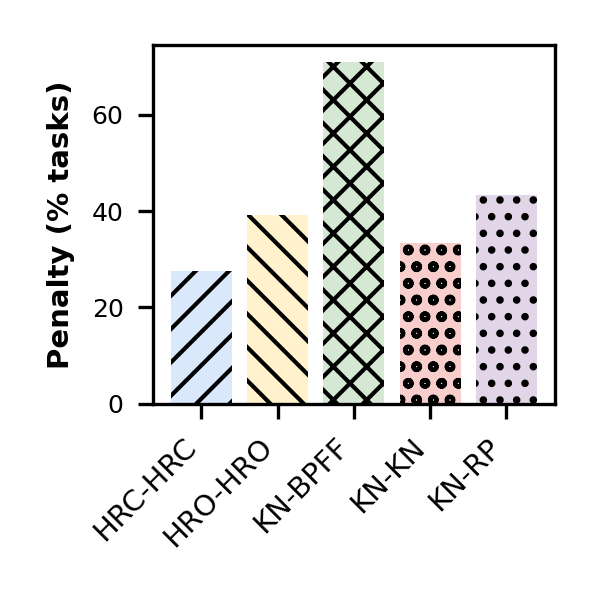
\includegraphics[width=0.155\linewidth]{6_Chapitre4/figures/eval/3-penalty-proportions.png}
    }
    \subfloat[Energy\label{figure:herocache-evaluation-full-energy-consumption}]{
        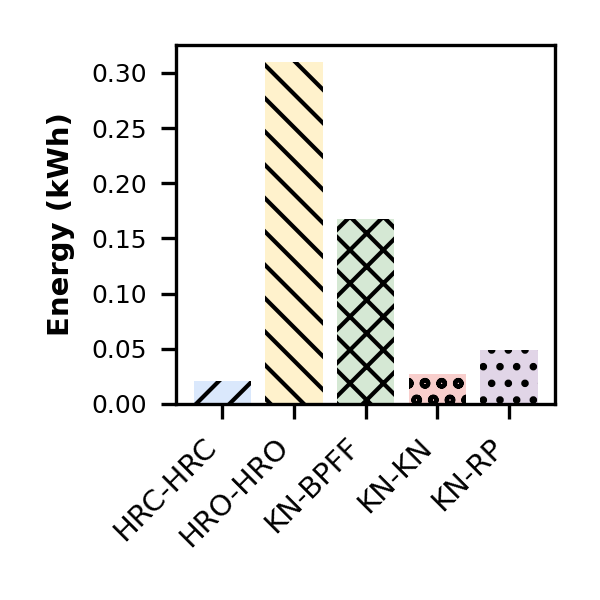
\includegraphics[width=0.155\linewidth]{6_Chapitre4/figures/eval/6-energy-consumption.png}
    }
    \subfloat[Consolidation\label{figure:herocache-evaluation-components-unused-nodes}]{
        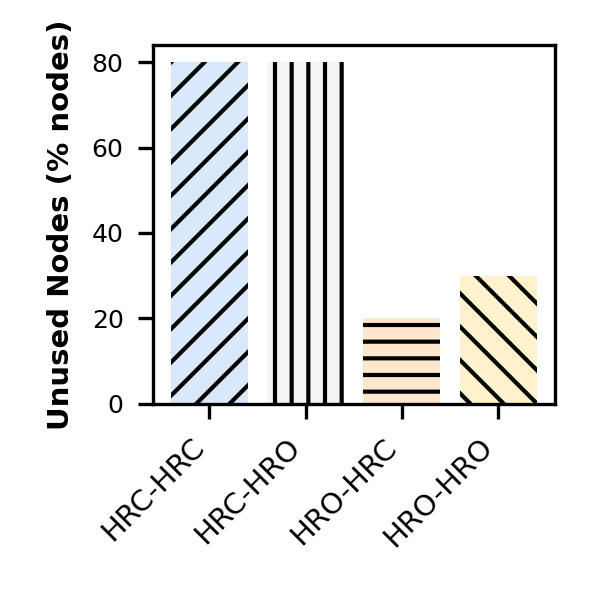
\includegraphics[width=0.155\linewidth]{6_Chapitre4/figures/eval-components/2-unused-nodes.png}
    }
    \subfloat[QoS\label{figure:herocache-evaluation-components-penalty}]{
        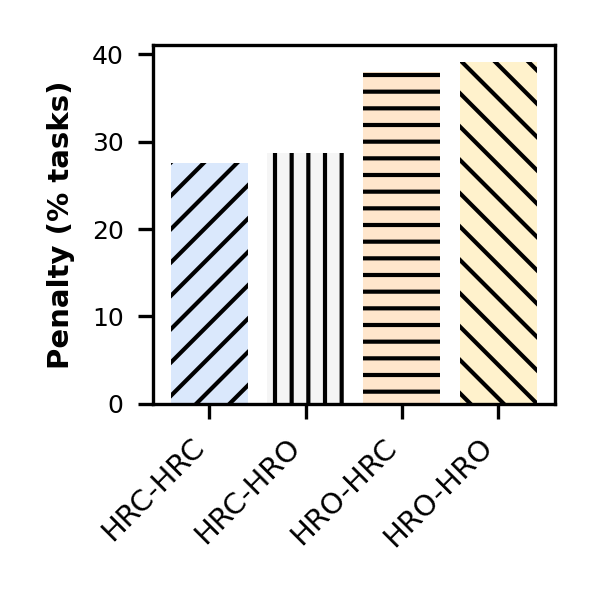
\includegraphics[width=0.155\linewidth]{6_Chapitre4/figures/eval-components/3-penalty-proportions.png}
    }
    \subfloat[Energy\label{figure:herocache-evaluation-components-energy-consumption}]{
        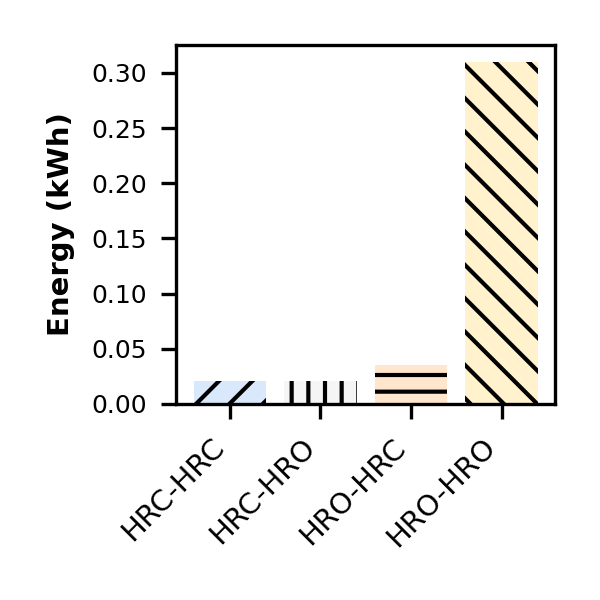
\includegraphics[width=0.155\linewidth]{6_Chapitre4/figures/eval-components/6-energy-consumption.png}
    }
    \caption{Evaluation -- Comparison against baselines (a-c) and impact of individual components (d-f)}
    \label{figure:herocache-evaluation}
\end{figure*}

\subsection{Protocole expérimental}

\textbf{Métadonnées de caractérisation hors-ligne}. Pour évaluer notre contribution, nous avons effectué des mesures pour trois applications IDS (voir Section~\ref{section:herocache-characterization-workloads}). Ces applications consistent en différentes fonctions de prétraitement et d'inférence qui ont été mises en œuvre sur du matériel hétérogène (voir Section~\ref{section:herocache-characterization-platforms}). Ces métadonnées ont servi d'entrée à un simulateur~\footnote{\href{https://github.com/b-com/HeROsim}{https://github.com/b-com/HeROsim}} que nous avons construit en utilisant SimPy~\cite{simpy}.

\textbf{L'ordonnanceur en ligne}. Nous avons généré des scénarios synthétiques en modélisant les demandes des utilisateurs comme un processus de Poisson, suivant une distribution uniforme entre les invocations d'applications, comme indiqué dans~\cite{9928755}. En modifiant le paramètre $\lambda$ du processus de Poisson, nous pouvons générer diverses traces avec différents taux de requêtes par seconde (RPS). Nous avons envisagé un scénario avec 10 nœuds de bordure communiquant via une connectivité 4G (LTE). La largeur de bande pour la 4G LTE dépend de divers facteurs allant de la couverture de l'antenne à la qualité de service du fournisseur de services de communication, en passant par la qualité du récepteur. Nous avons choisi d'utiliser des valeurs générales de 100 Mbps (12,5~MB/s). Les paquets TCP à analyser ont une taille de 1,5~KB et sont envoyés par lots de 100 unités aux applications IDS. Cela donne un taux de 83~RPS dans notre scénario, pour 10 minutes de requêtes d'utilisateurs. 

Les pondérations pour les décisions de mise à l'échelle automatique (équation~\ref{eq:herocache-scale-cost-function}) ont été fixées à $k_{CP} = \frac{3}{8}$, $k_{TT} = \frac{3}{8}$, $k_{EC} = \frac{1}{8}$ et $k_{HP} = \frac{1}{8}$. Les pondérations pour les décisions d'ordonnanceur (équation~\ref{eq:herocache-scheduling-cost-function}) ont été fixées à $k_{QP} = \frac{2}{3}$, $k_{EC} = \frac{0.5}{6}$ et $k_{TC} = \frac{1.5}{6}$. Nous utilisons des valeurs inspirées de \cite{herofake} afin d'être comparables.

Pour éviter une forme d'"emballement" (\textit{thrashing}) où les répliques sont créées et détruites en boucle lorsque la concurrence dans le système est très proche du seuil de concurrence, l'autoscaler applique un temps de maintien en vie faible qui empêche le retrait d'une réplique qui a été récemment allouée. Nous avons fixé ce temps de maintien en vie à 30 secondes, ce qui est la valeur par défaut dans Knative.

Dans nos expériences, nous permettons d'évaluer l'autoscaler et l'ordonnanceur séparément afin de mieux comprendre leur comportement. Nous avons évalué différentes combinaisons pour montrer quelle partie de chaque politique est pertinente pour relever les différents défis de notre problème. Nous avons mis en œuvre trois autoscalers dans notre simulateur :

\begin{itemize}
    \item HeROcache (HRC) -- Notre politique de mise à l'échelle automatique repose sur la mise en cache d'images de fonctions sur les nœuds edge et tente de prélever des images de fonctions pour satisfaire les dépendances avant le déploiement dans le DAG d'applications ;
    \item HeROfake (HRO)~\cite{herofake} -- Applique une politique similaire à HRC, mais ne tient pas compte des coûts de stockage : il n'utilise pas le cache d'image local du nœud lors de l'instanciation des répliques de fonctions, et n'effectue pas non plus la recherche préalable des images de fonctions en fonction du DAG de leur application ;
    \item Knative (KN)~\cite{sureshENSUREEfficientScheduling2020} -- Nous avons modélisé le comportement de l'autoscaler Knative au mieux de nos connaissances. Il déploie les répliques de fonctions sur le nœud le plus disponible, \textit{i.e.} il applique l'équilibrage de la charge.
\end{itemize}

En plus de ces autoscalers, nous avons utilisé quatre ordonnanceurs :

\begin{itemize}
    \item HeROcache (HRC) -- Notre politique d'ordonnancement sélectionne les demandes des utilisateurs entrants en fonction de l'échéance la plus proche afin de maximiser la qualité de service. Elle tient compte de la latence de communication prévue et sélectionne une réplique en fonction des exigences de temps de réponse dictées par la demande de l'utilisateur ;
    \item HeROfake (HRO)~\cite{herofake} -- Applique une politique similaire à HRC, mais ne tient pas compte des coûts de stockage : il ne prédit pas la latence des communications dans le DAG de l'application ;
    \item Knative (KN)~\cite{knative} -- Knative considère les plateformes d'exécution comme homogènes et n'applique pas la QoS. Les répliques sont triées en fonction du nombre de demandes en cours d'exécution ; la réplique ayant la file d'attente la plus courte est sélectionnée ;
    \item Bin-Packing First Fit (BPFF)~\cite{wangPeekingCurtainsServerlessb} -- Les tâches sont consolidées sur le nombre minimum de nœuds et de plateformes d'exécution. Les nœuds sont triés en fonction de la mémoire disponible ; la première réplique de fonction sur un nœud ayant de la mémoire disponible sera sélectionnée pour la demande de l'utilisateur. BPFF est susceptible d'être la politique d'ordonnanceur pour AWS Lambda ;
    \item Random Placement (RP) -- Les tâches sont ordonnancées sur une réplique sélectionnée de manière aléatoire.
\end{itemize}

Le nom de chaque scénario se compose de deux parties divisées par un symbole de tiret. La première partie correspond à la politique d'autoscaler ; la deuxième partie correspond à la politique d'ordonnanceur (par exemple, HRC-KN signifie que nous avons utilisé l'autoscaler HeROcache avec l'ordonnanceur Knative).

Nous avons conçu une évaluation des performances en deux étapes : \\
(1) \textbf{Comparaison avec les politiques de base} : nous comparons HeROcache complet (HRC-HRC) à : (1) Knative complet (KN-KN), (2) HeROfake complet (HRO-HRO), (3) l'autoscaler Knative avec l'ordonnanceur BPFF (KN-BPFF), (4) l'autoscaler Knative avec l'ordonnanceur RP (KN-RP). \\
(2) \textbf{Impact des composants de HeROcache sur les performances globales} : nous discutons de l'impact individuel de l'autoscaler et de l'ordonnanceur dans différentes stratégies : (1) l'autoscaler HeROcache avec l'ordonnanceur HeROfake (HRC-HRO), et (2) l'autoscaler HeROfake avec le scheduler HeROcache (HRO-HRC), en les comparant aux versions complètes de HeROcache et HeROfake.

Nous évaluons HeROcache sur la base de trois mesures : (1) le nombre de nœuds inutilisés dans l'infrastructure, qui mesure le niveau de consolidation atteint ; (2) les pénalités de qualité de service, qui expriment la capacité de notre stratégie à répondre aux exigences des utilisateurs ; (3) la consommation d'énergie, qui est un défi important à l'edge avec des ressources limitées.

\subsection{Analyse des résultats}

\subsubsection{Comparaison aux politiques de base}

\textbf{Consolidation des tâches}. La figure~\ref{figure:herocache-evaluation-full-unused-nodes} montre que notre combinaison d'autoscaler et d'ordonnanceur réalise la meilleure consolidation des tâches, en utilisant seulement 20\% de l'infrastructure edge pour l'exécution du scénario. Knative se comporte comme prévu, en répartissant la charge sur l'ensemble de l'infrastructure. Notez que BPFF sous Knative produit des résultats légèrement différents : comme les files d'attente des tâches sont maximisées, l'autoscaler n'a pas besoin d'allouer autant de répliques. Dans ce scénario, si les nœuds de bordure inutilisés étaient mis hors tension au lieu de rester inactifs, notre stratégie permettrait au fournisseur de services d'économiser près de 100 Wh (soit 80\% de l'énergie statique et plus de 83\% de l'énergie totale) en mettant hors tension 80\% de l'infrastructure, tout en garantissant le temps de réponse de l'application pour 72\% des demandes des utilisateurs.

\textbf{Qualité de service}. La figure~\ref{figure:herocache-evaluation-full-penalty} illustre la pertinence de la prise en compte de l'hétérogénéité des ressources. En effet, notre politique parvient à maintenir les violations de la qualité de service à 27,5\% tout en laissant 80\% de l'infrastructure inutilisée. Knative viole un peu plus de 30\% de la QoS des demandes des utilisateurs tout en répartissant la charge sur tous les nœuds de bordure disponibles, ce qui est contre-intuitif. Cela s'explique par les dépendances entre les tâches que Knative ne prend pas en compte. En conséquence, les tâches communiquent sur un réseau de stockage lent. Bien que les tâches dans Knative passent moins de temps dans la file d'attente, elles présentent toujours une latence plus élevée que dans HeROcache. Lors de l'utilisation de la politique BPFF, les violations atteignent presque 70\% : dans cette situation, les files d'attente des répliques sont trop longues pour que les tâches puissent être achevées dans les délais impartis. À titre de comparaison, Knative utilisant l'ordonnanceur RP maintient les violations de la QoS autour de 50\%. HeROfake génère 39\% de violations de la qualité de service.

Notre politique maintient la proportion de démarrages à froid en dessous de 0,011\% des demandes des utilisateurs, alors que Knative souffre de 4 fois plus de démarrages à froid. Dans HeROcache, le cache d'images local au nœud est utilisé dans 33\% des initialisations de fonctions, ce qui réduit les délais d'initialisation de 17,6\%.
Avec HeROcache, 30\% des tâches parviennent à communiquer par le biais du stockage local au niveau du nœud, ce qui accélère l'exécution de l'application en réduisant la latence des communications de 88,4\%.

\textbf{Consommation d'énergie}. La figure~\ref{figure:herocache-evaluation-full-energy-consumption} montre que HeROcache parvient à réduire la consommation d'énergie dynamique d'un tiers : avec un makespan de 1505 secondes pour le scénario, l'infrastructure consomme 0,0088 kWh, contre 0,0266 kWh pour 2193 secondes de temps d'exécution sous Knative. Non seulement la stratégie de consolidation de HeROcache permet d'appliquer des politiques de mise hors tension susceptibles de réduire considérablement les besoins en énergie statique pour l'exécution d'applications IDS en périphérie, mais en sélectionnant des plates-formes d'exécution adéquates, elle réduit également la consommation globale de la grappe en périphérie. HeROfake consomme le plus d'énergie (0,31 kWh) en raison d'un temps d'exécution beaucoup plus long pour le scénario.

\subsubsection{Impact des composants individuels}

\textbf{Consolidation des tâches}. La figure~\ref{figure:herocache-evaluation-components-unused-nodes} montre que les stratégies qui ne tiennent pas compte des coûts de stockage ne parviennent pas à consolider les tâches aussi bien que HeROcache : HRO-HRC et HRO-HRO utilisent respectivement 80\% et 70\% de l'infrastructure. Nous expliquons ces résultats de la manière suivante : les dépendances n'étant pas satisfaites à temps, la charge continue d'augmenter pour les différentes fonctions, ce qui conduit l'autoscaler à augmenter le nombre de répliques, enrôlant ainsi plus de nœuds pour la durée du scénario.

\textbf{Qualité de service}. La figure~\ref{figure:herocache-evaluation-components-penalty} illustre la conséquence du point précédent : Les pénalités de qualité de service sont plus élevées avec un autoscaler qui ne tient pas compte des délais introduits par l'extraction des images des fonctions et les communications des fonctions. Bien que HRO-HRC soit conscient de l'hétérogénéité du matériel et des requêtes, il termine tout de même avec 37,9\% des applications qui ne respectent pas leur délai.

\textbf{Consommation d'énergie}. La figure~\ref{figure:herocache-evaluation-components-energy-consumption} montre que, bien que HRO-HRC alloue 70\% de l'infrastructure, il parvient à maintenir une consommation d'énergie presque aussi faible que HRC-HRC. Cela s'explique par le fait qu'il a choisi les nœuds les moins gourmands en énergie, au prix de pénalités qu'il ne pouvait pas prévoir puisqu'il n'est pas conscient du stockage.

\textbf{Note sur la complexité} : HeROcache utilise une technique d'optimisation gourmande comparable à HeROfake. Dans HeROcache, la complexité est limitée par le nombre d'applications $A$, leur taille $f_{a}$ et la taille de l'infrastructure $N$ (équation~\ref{eq:herocache-complexity-autoscaler}) : dans le pire des cas où toutes les ressources sont disponibles, l'autoscaler parcourt l'ensemble de l'infrastructure $N$ pour évaluer chaque nœud en vue de la création de répliques.

\begin{equation}
    \mathcal{O}_{autoscaling}(A \cdot f_{a} \cdot N)
\label{eq:herocache-complexity-autoscaler}
\end{equation}

Comme l'ordonnanceur travaille avec des répliques déjà créées $R_{f}$ de fonctions, sa complexité est moindre (équation~\ref{eq:herocache-complexity-scheduler}).

\begin{equation}
    \mathcal{O}_{scheduling}(A \cdot f_{a} \cdot R_{f})
\label{eq:herocache-complexity-scheduler}
\end{equation}

Comme notre étude de cas actuelle implique un sous-ensemble limité de fonctions IDS avec un nombre raisonnable de nœuds edge, l'extensibilité n'a pas posé de problème. Toutefois, ces frais généraux devraient être pris en compte pour des déploiements plus larges de différentes études de cas. Ces frais généraux n'ont pas été mesurés en simulation. Toutefois, comme l'autoscaler fonctionne de manière périodique, la fréquence de la période pourrait être réglée pour ajuster l'algorithme en fonction des besoins du fournisseur de services. L'ordonnanceur est appelé au moment des demandes des utilisateurs et pourrait être réparti sur les nœuds si la charge est trop lourde à gérer.

\section{Travaux connexes}
\label{section:herocache-sota}

Des travaux antérieurs se sont concentrés sur les plates-formes de mise à l'échelle automatique pour le déploiement de tâches de courte durée, comprises dans des applications présentant des modèles de charge imprévisibles (voir Tableau~\ref{table:herocache-sota}).

Parmi ces travaux, \cite{smithFaDOFaaSFunctions2022} propose un orchestrateur conscient des données, mais ne tient pas compte de l'effet boule de neige des retards dans les chaînes de fonctions. \cite{zhangFIRSTExploitingMultiDimensional2023} ne prend pas en charge l'ordonnanceur de ces chaînes de fonctions.
Toutes ces contributions considèrent une infrastructure homogène \cite{bhasiCypressInputSizesensitive2022, zijunFassflowEfficient2022, smithFaDOFaaSFunctions2022, zhangFIRSTExploitingMultiDimensional2023, abdiPaletteLoadBalancing2023}. Cela n'est pas représentatif de notre cas d'utilisation, où les appareils edge sont très hétérogènes. HeROfake~\cite{herofake} exploite l'hétérogénéité matérielle dans sa politique d'orchestration, mais n'intègre pas les dépendances inter-fonctions ni la mise en cache d'images dans son modèle de coût. Elle a été choisie à des fins d'évaluation pour souligner la nécessité de prendre en compte ces coûts.
Certaines de ces contributions optimisent la consommation d'énergie au niveau de l'autoscaler \cite{bhasiCypressInputSizesensitive2022, zhangFIRSTExploitingMultiDimensional2023}. Toutefois, ils se concentrent sur la partie dynamique de la consommation d'énergie : ils ne tiennent pas compte de l'impact possible de la consolidation sur la consommation d'énergie statique. Nous soutenons que les fournisseurs de services devraient chercher à consolider les tâches afin de mettre hors tension le plus grand nombre de nœuds possible, ce qui réduirait considérablement les besoins énergétiques globaux de l'infrastructure.
Dans \cite{fuerstIluvatarFastControl2023}, les auteurs ont étudié les différents frais généraux infligés par l'orchestration serverless. Cet élément n'a pas été pris en compte dans notre étude, car nous visons une infrastructure edge de taille limitée pour le déploiement d'une seule application.

\section{Conclusion et perspectives}
\label{section:herocache-conclusion}

Dans ce travail, nous avons présenté une politique d'allocation et d'ordonnanceur pour le serverless à l'edge. Cette politique cherche à optimiser le déploiement d'applications sensibles au temps pour la qualité de service sur des dispositifs à énergie limitée. En tirant parti de la caractérisation de la charge de travail, de l'hétérogénéité du matériel et des dispositifs de stockage locaux sur les nœuds edge, HeROcache consolide les applications et parvient à réduire les délais d'initialisation moyens de 17,6\% et les délais de communication de 88,4\%. Cela permet de réduire la consommation d'énergie statique de la plateforme de 80\% tout en maintenant moins de 28\% de violations de la qualité de service. Nous prévoyons de généraliser l'approche HeROcache pour des études de cas incluant plusieurs types d'applications sur des infrastructures à l'edge ou en nuage plus importantes. Dans ce cas, des stratégies d'apprentissage automatique ou des métaheuristiques pourraient être utilisées à des fins de mise à l'échelle.
